\documentclass[letterpaper,11pt]{article}
\pdfoutput=1 % if you are submitting a pdflatex (i.e. if you have  
% images in pdf, png or jpg format)
\usepackage{jheppub}
\usepackage[utf8]{inputenc} 
%\usepackage[T1]{fontenc} % if needed
%\usepackage[latin1]{inputenc}
\usepackage{graphicx}
\usepackage{amsmath}
\usepackage{amsfonts}
\usepackage{slashed}
\usepackage{amssymb}
\usepackage{hyperref}
\hypersetup{colorlinks=true, linkcolor=blue, citecolor=red, urlcolor=cyan, linktoc=page}
%\usepackage{cite}
\usepackage{xfrac}
\usepackage{empheq}
\usepackage{caption, subcaption}

\newcommand{\p}{\partial}
\newcommand{\oi}{\omega_i}
\newcommand{\oj}{\omega_j}
\newcommand{\ok}{\omega_k}
\newcommand{\ol}{\omega_\ell}
\newcommand{\oone}{\overline{\omega}_1}
\newcommand{\otwo}{\overline{\omega}_2}
\newcommand{\thi}{\theta_i}
\newcommand{\thj}{\theta_j}
\newcommand{\thk}{\theta_k}
\newcommand{\thl}{\theta_\ell}
\newcommand{\mc}{\mathcal}
\newcommand{\jm}{\ensuremath{j_{max}}}
\newcommand{\ob}{\overline{\omega}}
\newcommand{\oib}{\overline{\omega}_i}
\newcommand{\ojb}{\overline{\omega}_j}
\newcommand{\okb}{\overline{\omega}_k}
\newcommand{\ib}{\overline{i}}
\newcommand{\jb}{\overline{j}}
\newcommand{\kb}{\overline{k}}
\newcommand{\oal}{\omega_\alpha}
\newcommand{\obet}{\omega_{\beta}}
\newcommand{\ogam}{\omega_\gamma}

%%%%%%%%%%%%%%%%%%%%%%%%%%%%%%%%%%%%%%%%%
%%%%%%%%%%%%%%%%%%%%%%%%%%%%%%%%%%%%%%%%%

\title{Arbitrary Dimensions, Massive, Non-normalizable Time-Dependent BCs}

\abstract{}

%%%%%%%%%%%%%%%%%%%%%%%%%%%%%%%%%%%%%%%%%
%%%%%%%%%%%%%%%%%%%%%%%%%%%%%%%%%%%%%%%%%

\begin{document}
\maketitle
\flushbottom
\newpage

%%%%%%%%%%%%%%%%%%%%%%%%%%%%%%%%%%%%%%%%%
%%%%%%%%%%%%%%%%%%%%%%%%%%%%%%%%%%%%%%%%%

\section{Introduction}

%%%%%%%%%%%%%%%%%%%%%%%%%%%%%%%%%%%%%%%%%
%%%%%%%%%%%%%%%%%%%%%%%%%%%%%%%%%%%%%%%%%

\section{Perturbative Expansion}

The backreaction between the metric and the scalar field appears at second order in the perturbation,
\begin{align}
A_2' = - \mu \nu \left[ (\dot \phi_1 )^2 + (\phi_1')^2 + m^2 \phi_1^2 \sec^2 x \right] + \nu' A_2 / \nu
\end{align}
which can be directly integrated to give

\begin{align}
A_2 = -\nu \int^x_0 dy \, \mu \left( (\dot \phi_1 )^2 + (\phi_1')^2 + m^2 \phi_1^2 \sec^2 x \right) \, .
\end{align}
Furthermore, the first non-trivial contribution to the lapse in the boundary time gauge is

\begin{align}
\delta_2 = \int^{\pi/2}_x dy \, \mu \nu \left(  (\dot \phi_1 )^2 + (\phi_1')^2 \right) \, .
\end{align}
For convenience, we have also defined the functions
\begin{align}
\mu (x) = \left( \tan x \right)^{d-1} \quad \text{and} \quad \nu(x) = (d-1) / \mu ' \, .
\end{align}

To aide in evaluating integrals, we first derive the following identities: from the equation for the first-order time-dependent coefficients $c_i$,
\begin{align} 
\ddot c_i + \oi^2 c_i = 0 \quad \Rightarrow \quad \p_t \left(\dot c_i^2 + \oi^2 c_i^2 \right) = \p_t \mathbb C_i = 0 \, ;
\end{align}
from the equation definition of $\hat L$,
\begin{align}
\hat L e_j = -\frac{1}{\mu} \left( \mu e'_j \right)' + m^2 \sec^2 x e_j \quad \Rightarrow \quad \left( \mu e'_j \right)' = \mu \left( m^2 \sec^2 x - \omega_j^2 \right) e_j \, ;
\end{align}
from considering the expression $\left( \mu e'_i e_j \right)'$:
\begin{align}
\left( \mu e'_i e_j \right) ' = \left(m^2 \sec^2 x - \oi^2 \right) \mu e_i e_j + \mu e'_i e'_j \, ;
\end{align}
from permuting $i, j$ above and subtracting to give
\begin{align}
\frac{\left[ \mu (e'_i e_j \oj^2 - e_i e'_j \oi^2 ) \right]'}{(\oj^2 - \oi^2)} = \mu m^2 \sec^2 x e_i e_j + \mu e'_i e'_j \, .
\end{align}

The basis functions $e_j (x)$ are the solutions to the eigenvalue equation
\begin{align}
\hat L e_j(x) = \omega^2_j e_j(x) .
\end{align}
When considering normalizable solutions only, the basis functions become
\begin{align}
e_j(x) &= k_j \left( \cos(x) \right)^{\Delta^+} P_{j}^{(d/2 - 1, \Delta^+ - d/2)} \left( \cos (2x) \right) \\
k_j &= 2 \sqrt{\frac{(j + \Delta^+ /2) \Gamma(j+1) \Gamma(j+\Delta^+)}{\Gamma(j+d/2) \Gamma(j + \Delta^+ - d/2 + 1)}} \, ,
\end{align} 
with eigenvalues $\omega_j = 2j + \Delta^+$, $j \in \mathbb{Z}^*$, and $\Delta^+$ as the positive root of $\Delta ( \Delta - d ) = m^2$. On the other hand, for non-normalizable solutions with arbitrary frequency, the basis functions are
\begin{align}
\label{general basis}
E_\omega (x) =  \left( \cos(x) \right)^{\Delta_+} {_2F_1} \left(\frac{\Delta_+ + \omega}{2}, \frac{\Delta_+ - \omega}{2}, d/2 ; \sin^2 (x) \right) \, .
\end{align}

%%%%%%%%%%%%%%%%%%%%%%%%%%%%%%%%%%%%%%%%%
%%%%%%%%%%%%%%%%%%%%%%%%%%%%%%%%%%%%%%%%%

\section{$\mc O(\epsilon^3)$ Source Terms}
At third order in $\epsilon$, the equation for $\phi_3$ contains a source $S$ given by
\begin{align}
\ddot \phi_3 + \hat L \phi_3 = S = 2 (A_2 - \delta_2) \ddot \phi_1 + (\dot A_2 - \dot \delta_2) \dot\phi_1 + (A_2' -\delta_2' )\phi_1' + m^2 A_2 \phi_1 \sec^2 x \, .
\end{align}
Following the steps outlined in Appendix~\ref{source term derivation}, and employing the solution $c_i(t) = a_i \cos (\oi t + b_i) = a_i \cos \theta_i$, the source term becomes
\begin{align}
\label{general source}
S_\ell &=\frac{1}{4} \sum_{\substack{i,j,k \\ k \neq \ell}}^\infty \frac{a_i a_j a_k \ok}{\ol^2 - \ok^2} \Big[ Z^-_{ijk\ell} (\oi + \oj - 2\ok) \cos (\thi + \thj - \thk) - Z^-_{ijk\ell} (\oi + \oj + 2\ok) \cos (\thi + \thj + \thk) - \nonumber \\
%
&\qquad + Z^+_{ijk\ell} (\oi - \oj + 2\ok)  \cos(\thi - \thj + \thk) - Z^+_{ijk\ell} (\oi - \oj - 2\ok) \cos (\thi - \thj - \thk) \Big] \nonumber \\
%
& + \frac{1}{2}\sum_{\substack{i,j,k \\ i \neq j}}^\infty a_i a_j a_k \oj \left( H_{ijk\ell} + m^2 V_{jki\ell} - 2\ok^2 X_{ijk\ell} \right) \Big[ \frac{1}{\oi - \oj} \left( \cos (\thi - \thj - \thk)  + \cos(\thi - \thj + \thk) \right) \nonumber \\
%
& \qquad - \frac{1}{\oi + \oj} \left( \cos (\thi + \thj - \thk)  + \cos ( \thi + \thj + \thk) \right) \Big] \nonumber \\
%
& - \frac{1}{4} \sum_{i,j,k}^\infty a_i a_j a_k \Big[ \left( 2\oj \ok X_{ijk\ell} + m^2 V_{ijk\ell} \right)\cos(\thi + \thj - \thk) -  \left( 2\oj\ok X_{ijk\ell} - m^2 V_{ijk\ell} \right) \cos(\thi - \thj - \thk) \nonumber \\
%
& \qquad + \left(2\oj \ok X_{ijk\ell} + m^2 V_{ijk\ell} \right) \cos (\thi - \thj + \thk) - \left( 2\oj\ok X_{ijk\ell} - m^2 V_{ijk\ell} \right) \cos(\thi + \thj + \thk) \Big] \nonumber \\
%
& + \frac{1}{4} \sum_{i,j}^\infty a_i a_j a_\ell \ol \Big[ \tilde Z^-_{ij\ell} (\oi + \oj - 2\ol) \cos (\thi + \thj - \thl) - \tilde Z^-_{ij\ell} (\oi + \oj + 2\ol) \cos(\thi + \thj +  \thl) \nonumber \\
%
& \qquad + \tilde Z^+_{ij\ell} (\oi - \oj + 2\ol) \cos(\thi - \thj + \thl)  - \tilde Z^+_{ij\ell} (\oi - \oj - 2\ol) \cos( \thi - \thj - \thl)  \Big] \nonumber \\
%
& - \frac{1}{4} \sum_{i,j}^\infty a_i^2 a_j \left( H_{iij\ell} + m^2 V_{jii\ell} - 2\oj^2 X_{iij\ell} \right) \big[ \cos (2\thi - \thj) + \cos (2\thi + \thj) \big] \nonumber \\
%
& - \frac{1}{2} \sum_{i,j}^\infty a_i^2 a_j \left( H_{iij\ell} + m^2 V_{jii\ell} - 2\oj^2 X_{iij\ell} + 4\oi^2 \oj^2 P_{j\ell i} + 2\oi^2 (M_{j\ell i} + m^2 Q_{j\ell i}) \right) \cos \thj . \hspace{-0.2in}
\end{align} 

%%%%%%%%%%%%%%%%%%%%%%%%%%%%%%%%%%%%%%%%%
%%%%%%%%%%%%%%%%%%%%%%%%%%%%%%%%%%%%%%%%%

\section{Resonances From Normalizable Solutions}
\label{sec: norm res}
Consider the case where each of the basis functions are given by normalizable solutions. After time-averaging, resonant contributions come from the set of conditions
\begin{align}
\label{gen res}
\oi \pm \oj \pm \ok = \pm \ol \,
\end{align}
which separates into three distinct cases
\begin{align}
\oi + \oj + \ok &= \ol \qquad (+++) \\
\oi - \oj - \ok &= \ol \qquad (+--) \\
\oi + \oj - \ok &= \ol \qquad (++-)
\end{align}

%%%%%%%%%%%%%%%%%%%%%%%%%%%%%%%%%%%%%%%%%

\subsection{$(+++)$}

These resonant contributions come from the condition $\oi + \oj + \ok = \ol$, and are of the form
\begin{align}
S_\ell = \underbrace{\sum_{i=0}^\infty \sum_{j=0}^\infty \sum_{k=0}^\infty}_{\oi + \oj + \ok = \, \ol} \Omega_{ijk\ell} \, a_i a_j a_k \cos \left( \thi + \thj + \thk \right) + \ldots \, ,
\end{align}
where
\begin{align}
\label{omega}
\Omega_{ijk\ell} &= -\frac{1}{12}H_{ijk\ell} \frac{\oj (\oi + \ok +2\oj)}{(\oi + \oj)(\oj + \ok)} - \frac{1}{12} H_{ikj\ell} \frac{\ok (\oi + \oj + 2\ok)}{(\oi + \ok)(\oj + \ok)}- \frac{1}{12} H_{jik\ell} \frac{\oi (\oj + \ok +2\oi)}{(\oi + \oj)(\oi + \ok)} \nonumber \\
%
& \quad - \frac{m^2}{12} V_{ijk\ell} \left( 1 + \frac{\oj}{\oj + \ok} + \frac{\oi}{\oi + \ok} \right) - \frac{m^2}{12} V_{jki\ell} \left( 1 + \frac{\oj}{\oi + \oj} + \frac{\ok}{\oi + \ok} \right) \nonumber \\
%
& \quad - \frac{m^2}{12} V_{kij\ell} \left( 1 + \frac{\oi}{\oi + \oj} + \frac{\ok}{\oj + \ok} \right)  + \frac{1}{6} \oj \ok X_{ijk\ell} \left( 1 + \frac{\oj}{\oi + \ok} + \frac{\ok}{\oi + \oj} \right) \nonumber \\
%
& \quad + \frac{1}{6} \oi \ok X_{jki\ell} \left( 1 + \frac{\oi}{\oj + \ok} + \frac{\ok}{\oi + \oj} \right) + \frac{1}{6} \oi \oj X_{kij\ell} \left( 1 + \frac{\oi}{\oj + \ok} + \frac{\oj}{\oi + \ok} \right) \nonumber \\
%
& \quad - \frac{1}{12} Z^-_{ijk\ell} \left( \frac{\ok}{\oi + \oj} \right) - \frac{1}{12} Z^-_{ikj\ell} \left( \frac{\oj}{\oi + \ok} \right) - \frac{1}{12} Z^-_{jki\ell}  \left( \frac{\oi}{\oj + \ok} \right) \, .
\end{align}

%%%%%%%%%%%%%%%%%%%%%%%%%%%%%%%%%%%%%%%%%

\subsection{$(+--)$}

These contributions arise from the condition $\oi - \oj - \ok = \ol$, are of the form
\begin{align}
S_\ell = \sum_{j=0}^\infty \sum_{k=0}^\infty \Gamma_{(j + k + \ell + \Delta^+) jk\ell} \, a_j a_k a_{(j+k+\ell + \Delta^+)} \cos \left( \theta_{(j+k+\ell + \Delta^+)} - \thj - \thk \right) + \ldots \, ,
\end{align}
where
\begin{align}
\label{gamma}
\Gamma_{ijk\ell} &= \frac{1}{4} H_{ijk\ell} \frac{\oj (\ok - \oi + 2\oj)}{(\oi - \oj)(\oj + \ok)} + \frac{1}{4} H_{jki\ell} \frac{\ok (\oj - \oi + 2\ok)}{(\oi - \ok)(\oj + \ok)} + \frac{1}{4} H_{kij\ell} \frac{\oi (\oj + \ok - 2\oi)}{(\oi - \oj)(\oi - \ok)} \nonumber \\
% 
& \quad -\frac{1}{2} \oj \ok X_{ijk\ell} \left( \frac{\ok}{\oi - \oj} + \frac{\oj}{\oi - \ok} - 1\right) + \frac{1}{2} \oi \ok X_{jki\ell} \left( \frac{\ok}{\oi - \oj} + \frac{\oi}{\oj + \ok} - 1 \right) \nonumber \\
%
& \quad + \frac{1}{2} \oi \oj X_{kij\ell} \left( \frac{\oj}{\oi - \ok} + \frac{\oi}{\oj + \ok} -1 \right) + \frac{m^2}{4} V_{jki\ell} \left( \frac{\oj}{\oi - \oj} + \frac{\ok}{\oi - \ok} -1\right) \nonumber \\
%
& \quad - \frac{m^2}{4} V_{kij\ell} \left( \frac{\oi}{\oi - \oj} + \frac{\ok}{\oj + \ok} + 1\right) - \frac{m^2}{4} V_{ijk\ell} \left( \frac{\oi}{\oi - \ok} + \frac{\oj}{\oj + \ok} + 1 \right) \nonumber \\
%
& \quad + \frac{1}{4} Z^-_{kji\ell} \left( \frac{\oi}{\oj + \ok}\right) - \frac{1}{4} Z^+_{ijk\ell} \left( \frac{\ok}{\oi - \oj} \right) - \frac{1}{4} Z^+_{jki\ell} \left( \frac{\oj}{\oi - \ok}\right) \, .
\end{align}

%%%%%%%%%%%%%%%%%%%%%%%%%%%%%%%%%%%%%%%%%

\subsection{Naturally Vanishing Resonances}

It has been shown that when working in the interior gauge, \eqref{omega} and \eqref{gamma} for a massless scalar vanish by the orthogonality of the basis functions. Moreover, we are able to demonstrate that these continue to vanish (as they must) for massive scalars in the boundary gauge. This means that the dynamics of the perturbative system are determined only from the remaining resonance channel. When non-normalizable modes are introduced, we will see that all none of the resonance channels naturally vanish.

%%%%%%%%%%%%%%%%%%%%%%%%%%%%%%%%%%%%%%%%%

\subsection{$(++-)$}
\label{subs: ttf resonances}

These contributions arise from the resonant condition $\oi + \oj = \ok + \ol$, can be written as
\begin{align}
S_\ell &= T_\ell a^3_\ell \cos (\thl + \thl - \thl) + \sum_{i \neq \ell}^\infty R_{i \ell} \, a^2_i a_\ell \cos(\thi + \thl - \thi) \nonumber \\
& \qquad + \sum_{i \neq \ell}^\infty \sum_{j \neq \ell}^\infty S_{i j (i + j - \ell) \ell} \, a_i a_j a_{(i + j - \ell)} \cos(\thi + \thj - \theta_{i + j -\ell} ) + \ldots
\end{align}
where each of the coefficients is given by
\begin{align}
S_{ijk\ell} &= - \frac{1}{4} H_{kij\ell} \frac{\oi (\oj - \ok + 2\oi)}{(\oi - \ok)(\oi + \oj)} -\frac{1}{4} H_{ijk\ell} \frac{\oj (\oi - \ok + 2\oj)}{(\oj - \ok)(\oi + \oj)} - \frac{1}{4} H_{jki\ell} \frac{\ok ( \oi + \oj - 2\ok)}{(\oi - \ok)(\oj - \ok)} \nonumber \\
%
& \quad - \frac{1}{2} \oj \ok X_{ijk\ell} \left( \frac{\oj}{\oi - \ok} - \frac{\ok}{\oi + \oj} + 1 \right) - \frac{1}{2} \oi \ok X_{jki\ell} \left( \frac{\oi}{\oj - \ok} - \frac{\ok}{\oi + \oj} + 1 \right) \nonumber \\
%
& \quad + \frac{1}{2} \oi \oj X_{kij\ell} \left( \frac{\oi}{\oj - \ok} + \frac{\oj}{\oi - \ok} + 1 \right) - \frac{m^2}{4} V_{ijk\ell} \left( \frac{\oi}{\oi - \ok} + \frac{\oj}{\oj - \ok} + 1\right) \nonumber \\
%
& \quad + \frac{m^2}{4} V_{jki\ell} \left( \frac{\ok}{\oi - \ok} - \frac{\oj}{\oi + \oj} - 1 \right) + \frac{m^2}{4} V_{kij\ell} \left( \frac{\ok}{\oj - \ok} - \frac{\oi}{\oi + \oj} - 1 \right) \nonumber \\
%
& \quad + \frac{1}{4}  Z^-_{ijk\ell} \left( \frac{\ok}{\oi + \oj}\right)  + \frac{1}{4}  Z^+_{ikj\ell} \left( \frac{\oj}{\oi - \ok}\right) + \frac{1}{4} Z^+_{jki\ell} \left( \frac{\oi}{\oj - \ok} \right) \, ,
\end{align}
\begin{align}
R_{i\ell} &= \left(\frac{\oi^2}{\ol^2 - \oi^2} \right) \big( Y_{i\ell \ell i} - Y_{i\ell i \ell} + \ol^2 ( X_{i\ell i \ell} - X_{\ell i \ell i}) \big) + \left(\frac{\oi^2}{\ol^2 - \oi^2}\right) \big( H_{\ell i i\ell} + m^2 V_{ii\ell \ell} - 2\oi^2 X_{\ell i i \ell} \big) \nonumber \\
%
& - \left(\frac{\ol^2}{\ol^2 - \oi^2} \right) \big( H_{i\ell i \ell} + m^2 V_{\ell i i \ell} - 2\oi^2 X_{i\ell i\ell} \big) - \frac{m^2}{4}(V_{i\ell i \ell} + V_{ii\ell \ell} ) + \oi^2 \ol^2 (P_{ii\ell} - 2P_{\ell \ell i}) \nonumber \\
%
& - \oi\ol X_{i\ell i \ell} - \frac{3m^2}{2} V_{\ell ii \ell} - \frac{1}{2} H_{ii\ell \ell} + \ol^2 B_{ii\ell} - \oi^2 M_{\ell \ell i} - m^2 \oi^2 Q_{\ell \ell i} \, ,
\end{align}
\begin{align}
T_{\ell} &= \frac{1}{2} \ol^2 \left( X_{\ell \ell \ell \ell} + 4 B_{\ell \ell \ell} -2 M_{\ell \ell \ell} - 2m^2 Q_{\ell \ell \ell} \right) -\frac{3}{4} \left( H_{\ell \ell \ell \ell} + 3m^2 V_{\ell \ell \ell \ell} \right) \, . \hspace{1.0in}
\end{align}

%%%%%%%%%%%%%%%%%%%%%%%%%%%%%%%%%%%%%%%%%
%%%%%%%%%%%%%%%%%%%%%%%%%%%%%%%%%%%%%%%%%

\section{Resonances From Non-normalizable Modes}

{\bf Discuss falloff of A2 and delta2 with three NN modes, but don't calculate anything new. Mention overlap of NN and normalizable cases when omega(i) $\pm$ omega(j) = NN frequency. Then focus on two NN modes.}

We now consider the case when at least one of the $e_i(x), e_j(x), e_k(x)$ is a non-normalizable mode. Since the boundary condition has been set to be a single non-normalizable mode, any non-normalizable modes in the source term must exactly cancel; therefore, at least two of the modes must be non-normalizable. This assumption breaks some of the symmetries that contributed to the previous expressions for resonance channels, and so the resonance conditions must be re-examined starting from the source expression \eqref{general source}.

An important consideration is also the effect of non-normalizable modes on the perturbative expansion that leads to the source equations. Since non-normalizable solutions do not have well-defined norms, we do not know \emph{a priori} that the inner products described in Appendix~\ref{source term derivation} are still finite. To investigate this, consider the second-order metric function $A_2$
\begin{align}
A_2 &= - \nu \int^x_0 dy \, \mu \left( (\dot \phi_1)^2 + (\phi'_1)^2 + m^2 \phi_1^2 \sec^2 x \right) \, ,
\end{align}
in the limit of $x \to \pi/2$ when the scalar field is given by a generic superposition of normalizable and non-normalizable eigenfunctions:
\begin{align}
\phi_1 (t, x) &= \sum_\alpha e_\alpha \cos (\omega_\alpha t ) + \sum_i a_i e_i \cos (\omega_i t + b_i) \, .
\end{align}
Focusing on the position-dependence only, we find that
\begin{align}
\lim_{\tilde x \to 0} A_2 (\tilde x = \pi /2 - x) = \tilde{x}^{-\xi} \left( \frac{2 \tilde{x}^{2+d}}{2 - \xi} - \frac{\tilde{x}^d (1 + \left(\Delta^{-}\right)^2)}{\xi} \right)
\end{align}
where we have defined $\xi = \sqrt{d^2 + 4m^2}$. In the massless case, $\xi = d$ and all powers of $\tilde{x}$ are non-negative and thus the limit is finite; for tachyonic masses, $0 \leq \xi < d$ and the limit is again finite. However, for massive scalars, at least one of the terms above diverges as $\xi \to 0$. This case would require the addition of counter-terms in the bulk action to cancel such divergences -- we will not consider this case presently. Thus, we will restrict our discussion to $m^2 \leq 0$ to avoid these issues. A similar check on the near-boundary behaviour of $\delta_2$ shows that, in the massless case, the gauge condition $\delta_2 (t, x=\pi/2)$ remains unchanged by the addition of non-normalizable modes.

\subsection{Two Non-normalizable Modes with Equal Frequencies}

As a first case, let us assume that the two non-normalizable modes have equal, constant, and arbitrary frequencies, $\ob$. Applying the time-averaging procedure to the source $S_\ell$ once again eliminates all contributions except those that satisfy \eqref{gen res}. Since the basis onto which we are projecting is normalizable, we know that $\omega_\ell$ is given by $\omega_\ell = 2\ell + \Delta^{+}$. We are now free to choose any one of $\{\omega_i, \omega_j, \ok\}$ to be normalizable and consider when the resonance condition is satisfied. In particular, we find that the following combinations are resonant:
\begin{align}
\label{gen nn res 1}
\oi - \oj + \ok - \ol &= 0 \qquad \Rightarrow \qquad \text{either $\oi$ or $\ok$ is normalizable} \\
\oi + \oj - \ok - \ol &= 0 \qquad \Rightarrow \qquad \text{either $\oi$ or $\oj$ is normalizable} \\
\oi - \oj - \ok + \ol &= 0 \qquad \Rightarrow \qquad \text{either $\oj$ or $\ok$ is normalizable.}
\label{gen nn res 2}
\end{align}
When any of these resonance conditions is met, the remaining normalizable mode will have a frequency equal to $\ol$, collapsing all sums over frequencies so that
\begin{align}
S_\ell = \overline{T}_{\ell \ob} \, a_\ell A_{\ob}^2 \cos (\thl) \, ,
\end{align}
where the non-normalizable modes have constant amplitudes $A_{\ob}$. Collecting the appropriate terms in \eqref{general source}, and evaluating the each possible resonance (being careful not to violate restrictions placed on the sums), we find that
\begin{align}
\label{S:2NN}
\overline{T}_{\ell \ob} &=  \left( 1 - \delta_{\ol, \ob} \right)\Big[ \, \frac{1}{2} Z^-_{\ell\ob\ob\ell} \left( \frac{\ob}{\ol + \ob} \right) + \frac{1}{2} Z^+_{\ell\ob\ob\ell} \left( \frac{\ob}{\ol - \ob} \right)  + H_{\ell \ob \ob \ell} \left( \frac{\ob^2}{\ol^2 - \ob^2} \right) \nonumber \\
%
& - H_{\ob\ell\ob\ell} \left(\frac{\ol^2}{\ol^2 - \ob^2} \right) - m^2 V_{\ell \ob\ob\ell}  \left(\frac{\ol^2}{\ol^2 - \ob^2} \right) + m^2 V_{\ob\ob\ell\ell} \left( \frac{\ob^2}{\ol^2 - \ob^2} \right) + 2 X_{\ob\ob\ell\ell} \left( \frac{\ob^2 \ol^2}{\ol^2 - \ob^2} \right) \nonumber \\
%
&  - 2 X_{\ell\ell\ob\ob} \left( \frac{\ob^4}{\ol^2 - \ob^2} \right) \Big] + \ol^2 X_{\ob\ob\ell\ell}  - \ob^2 X_{\ell\ell\ob\ob} - \frac{3}{2} m^2 V_{\ell\ell\ob\ob} - \frac{1}{2} m^2 V_{\ob\ob\ell\ell}  - \frac{1}{2} H_{\ob\ob\ell\ell} \nonumber \\
%
& + \ol^2 \tilde{Z}^+_{\ob\ob\ell} - 2 \ob^2 \ol^2 P_{\ell\ell\ob} - \ob^2 \left( \ol^2 P_{\ell\ell \ob} - B_{\ell\ell\ob} \right) \, .
\end{align}

Notice that the Kronecker delta multiplying the terms in the square braces means that these terms will only contribute when $\ob \neq \ol$. Beginning from \eqref{general source}, only terms in the square braces that are proportional to $Z^{\pm}$ are limited in this way; the remaining terms have no such restriction. However, it can be shown that integral functions with permuted indices are equal when the non-normalizable frequency equals the normalizable frequency. Upon simplification, factors of $\ol^2 - \ob^2$ are canceled and the overall contribution to $T_{\ob \ell}$ from the terms in the braces is zero. Thus, these terms are grouped with those that have natural restrictions on the indices. 

In figures~\ref{fig:equal_frequency_m0} and~\ref{fig:equal_frequency_m-4_0}, we evaluate \eqref{S:2NN} for $\ell < 10$ over a variety of $\ob$ values first for a massless scalar, then for a tachyonic scalar.

\begin{figure}
\centering
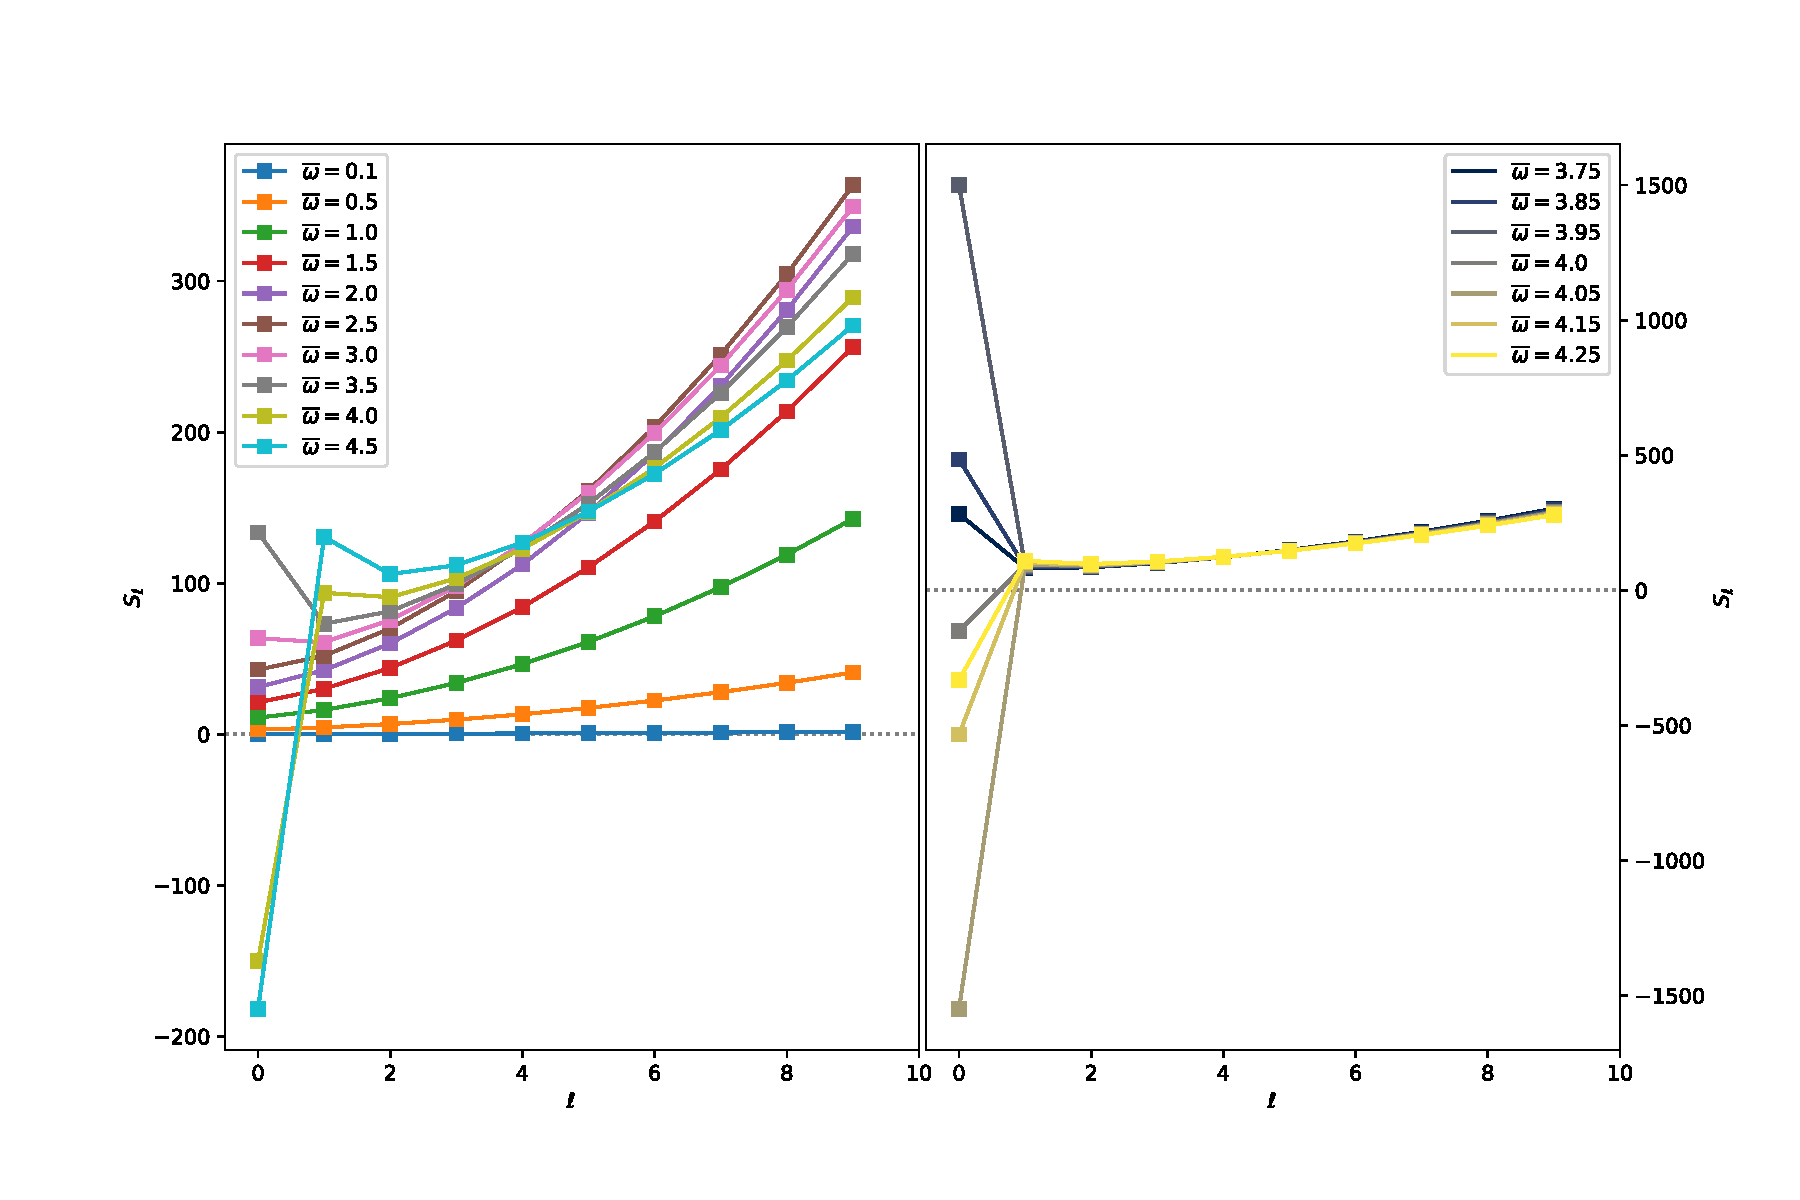
\includegraphics[width=\textwidth]{./figures/NN_equalfreq_sourceterms_m0_0+zoom}
\caption{{\it Left:} Evaluating $S_\ell$ (rescaled by the amplitudes) when $m^2 = 0$ for various choices of $\ob$. {\it Right}: The behaviour of $S_\ell$ for $\ob$ values near $\omega_0$.}
\label{fig:equal_frequency_m0}
\end{figure}

\begin{figure}[h]
\centering
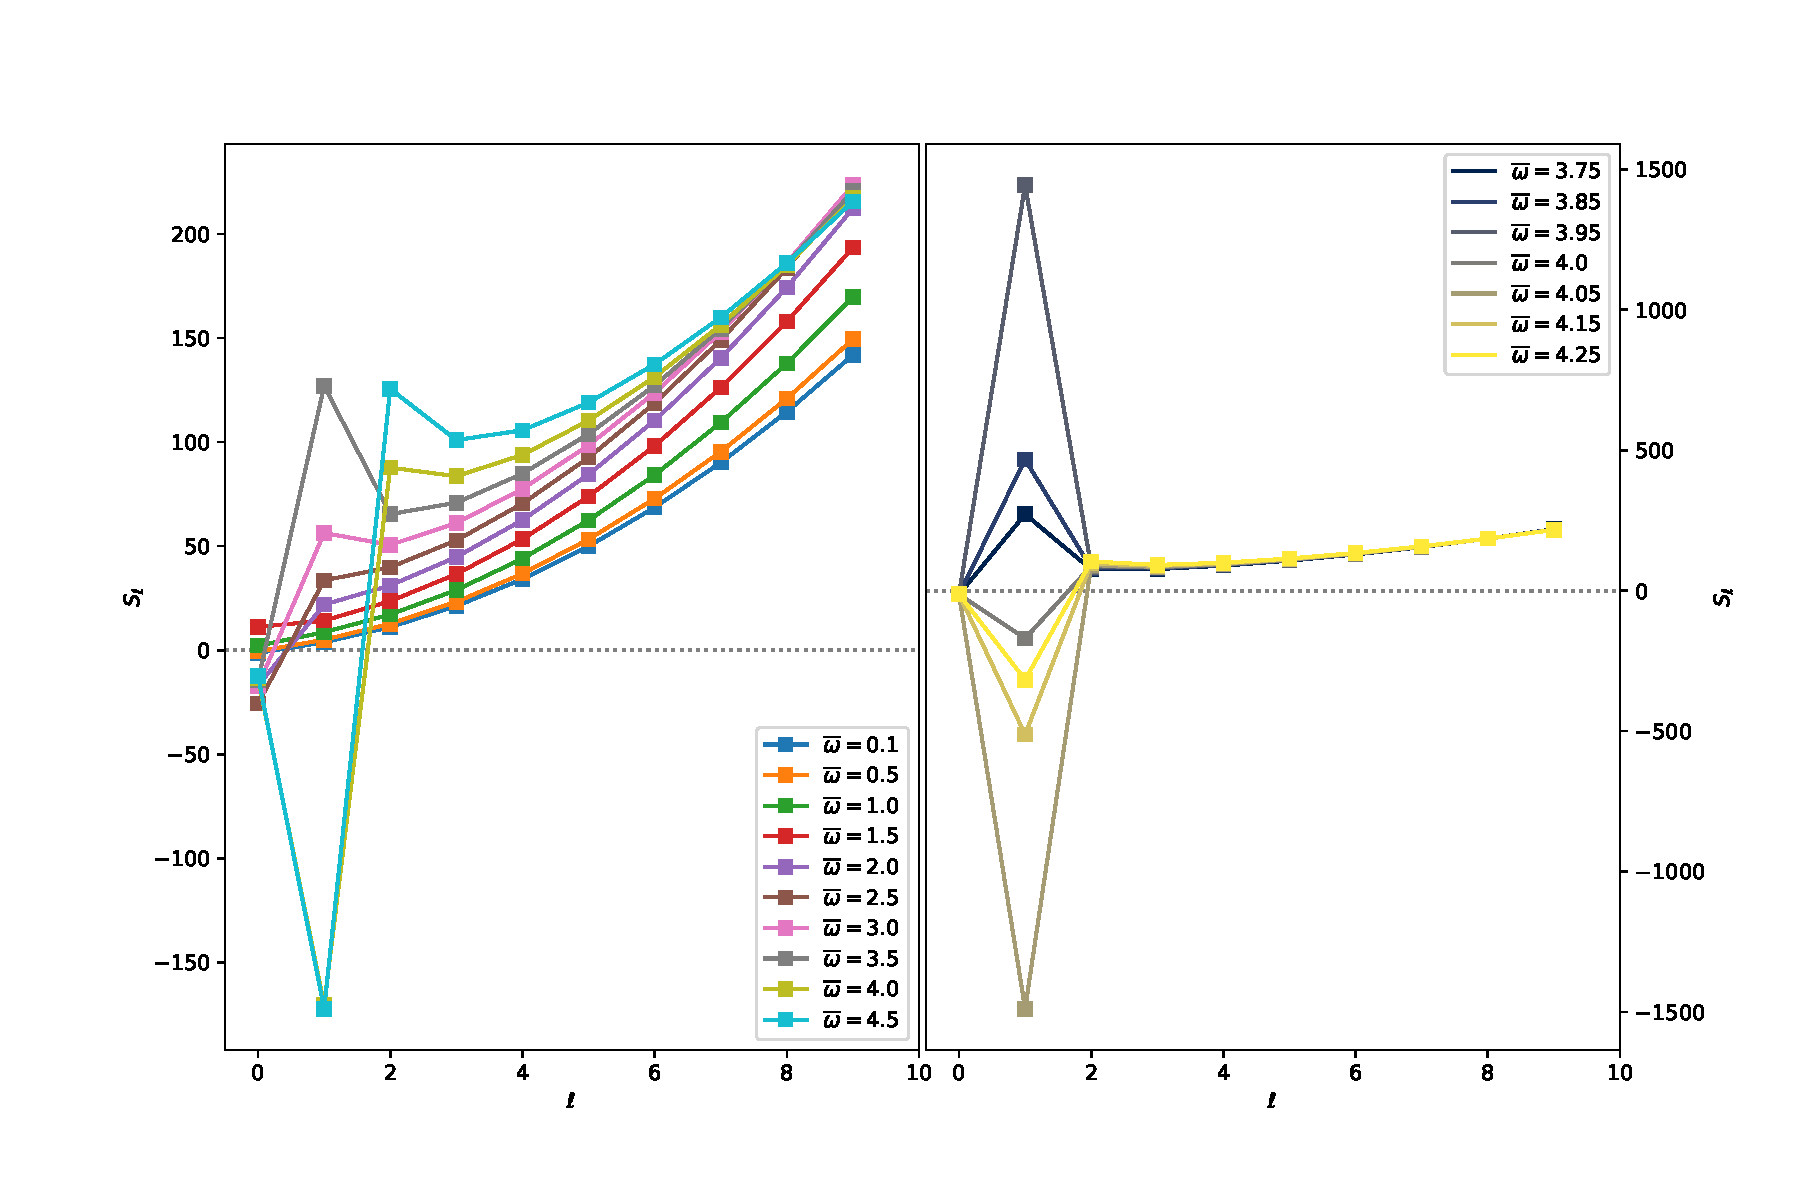
\includegraphics[width=\textwidth]{./figures/NN_equalfreq_sourceterms_m-4_0+zoom}
\caption{{\it Left:} Evaluating $\overline{T}_{\ell \ob}$ for a tachyon with $m^2 = -4.0$. {\it Right:} The behaviour of $S_\ell$ near $\omega_0 = \Delta^+ =  2$.}
\label{fig:equal_frequency_m-4_0}
\end{figure}

Other resonant contributions become possible for more restrictive values of the non-normalizable frequency, such as if $\ob$ is allow to be an integer. These contributions are not included here, but rather are discussed briefly in Appendix~\ref{more 2NN}.

\subsection{Special Values of Non-normalizable Frequencies}

Focus on non-arbitrary values of the non-normalizable frequencies.

\subsubsection{Add to an integer}
\label{ssec: add to integer}

Choose two of the modes to be non-normalizable with frequencies $\oone$ and $\otwo$ that add to give an integer: $\oone+ \otwo = 2n$ where $n = 1, 2, 3, \ldots$ (note that the $n = 0$ case means that both $\omega_1$ and $\omega_2$ would need to be zero by the positive-frequency requirement and so would not contribute). Furthermore, either frequency need not be an integer and therefore the difference $|\oone - \otwo|$ will not be an integer. 

When we consider possible resonance channels, we see that resonances can be grouped into
\begin{align}
\label{all pluses}
(++): \; \omega_I + 2n &= \omega_\ell \quad I \in \{i,j,k\} \; \forall \; \ell \geq n \\
(+-): \, \omega_I - 2n &=\omega_\ell \quad I \in \{i,j,k\} \; \forall \; n
\end{align}
for any $m^2_{BF} \leq m^2 < 0$. However, for a massless scalar, we have an additional channel
\begin{align}
\label{minus plus}
(-+): \, -\omega_I + 2n = \omega_\ell \quad I \in \{i,j,k\} \; \forall \; n \geq \ell + d
\end{align}
Adding the channels together, the total source term is
\begin{align}
\label{add to integer}
S_\ell &=\Theta \left( \ell - n \right)  \overline{R}^{(++)}_{(\ell - n) 1 2 \ell} \cos \left( \theta_{(\ell - n)} + 2nt \right) + \overline{R}^{(+-)}_{(\ell + n) 1 2 \ell } \cos\left( \theta_{(\ell + n)} - 2nt \right) \nonumber \\
%
& \quad + \Theta\left( n - \ell - d \right) \delta_{m^2} \overline{R}^{(-+)}_{(n - \ell - d) 1 2 \ell} \cos \left( \theta_{(n - \ell - d)} + 2nt \right) + \overline{T}_{12\ell} \cos \left( \theta_\ell \right) \, ,
\end{align}
where the Heaviside step function $\Theta(x)$ enforces the restrictions on the indices in \eqref{all pluses} and \eqref{minus plus} and the Kronecker delta is again employed to denote that terms in $\overline{R}^{(-+)}$ only contribute to the massless case.

In the following expressions, the sum over all $\oone$, $\otwo$ such that $\oone + \otwo = 2n$ is implied, and only the restrictions on individual frequencies are included. Examining each channel in \eqref{add to integer} individually, we find that
\begin{align}
\label{R1}
\overline{R}^{(++)}_{i 1 2 \ell} &= - \frac{1}{4} \sum_{\otwo \neq \ol} \frac{\otwo}{\ol - \otwo} Z^{-}_{i12\ell} - \frac{1}{4} \sum_{\oone \neq \ol} \frac{\oone}{\ol - \oone} Z^{-}_{i21\ell} - \frac{1}{8n} \sum \left( \ol - 2n \right) Z^-_{12i\ell} \nonumber \\
%
& - \frac{1}{4} \sum_{\oi \neq \oone} \frac{1}{\ol - \otwo} \Big[ \oone \left( H_{i12\ell} + m^2 V_{12i\ell} - 2 \otwo^2 X_{i12\ell} \right) + (\ol - 2n) \left( H_{1i2\ell} + m^2 V_{i21\ell} - 2\otwo^2 X_{1i2\ell} \right)\Big] \nonumber \\
%
& - \frac{1}{4} \sum_{\oi \neq \otwo} \frac{1}{\ol - \oone} \Big[ \otwo \left( H_{i21\ell} + m^2 V_{21i\ell} - 2\oone^2 X_{i21\ell} \right) + (\ol - 2n) \left( H_{2i1\ell} + m^2 V_{i12\ell} - 2\oone^2 X_{2i1\ell} \right) \Big] \nonumber \\
%
& - \frac{1}{8n} \sum_{\oone \neq \otwo} \Big[ \oone H_{21i\ell} + \otwo H_{12i\ell} + m^2 \left( \oone V_{1i2\ell} + \otwo V_{2i1\ell} \right) - \left( \ol - 2n \right)^2 \left(\oone X_{21i\ell} + \otwo X_{12i\ell} \right) \Big] \nonumber \\
%
& + \frac{1}{2} \sum \Big[ \oone\otwo X_{i12\ell} + \left( \ol - 2n \right)\left( \oone X_{21i\ell} + \otwo X_{12i\ell} \right) - \frac{m^2}{2} \left( V_{i12\ell} + V_{i21\ell} + V_{12i\ell} \right) \Big]
\end{align}
The notation $X_{i12\ell}$ corresponds to evaluating $X_{ijk\ell}$ with $\omega_j = \oone$ and $\omega_k = \otwo$. 

Next, we find that
\begin{align}
\label{R2}
\overline{R}_{i12\ell}^{(+-)} &= - \frac{1}{4} \sum \Big[ \frac{(\ol + 2n)}{2n} Z^-_{12i\ell} + 2 (\ol + 2n) \left( \oone X_{21i\ell} + \otwo X_{12i\ell} \right) \nonumber \\
%
& -\frac{\oone}{(\ol + \otwo)} \left( H_{i12\ell} + m^2 V_{12i\ell} - 2 \otwo^2 X_{i12\ell} \right) + \frac{(\ol + 2n)}{(\ol + \otwo)} \left( H_{1i2\ell} + m^2 V_{i21\ell} - 2\otwo^2 X_{1i2\ell} \right)  \nonumber \\
%
&- \frac{\otwo}{(\ol + \oone)} \left( H_{i21\ell} + m^2 V_{21i\ell} - 2\oone^2 X_{i21\ell} \right) + \frac{(\ol + 2n)}{(\ol + \oone)} \left(H_{2i1\ell} + m^2 V_{i12\ell} - 2\oone^2 X_{2i1\ell} \right)  \nonumber \\
%
&  - 2 \oone\otwo X_{i12\ell} + m^2 \left( V_{12i\ell} + V_{i12\ell} + V_{i21\ell} \right) \Big] + \frac{1}{4} \sum_{\otwo \neq \ol} \frac{\oone\otwo(\ol + 2n)}{\ol + \otwo} \left( X_{21i\ell} - X_{\ell i 12} \right) \nonumber \\
%
& + \frac{1}{4} \sum_{\oone \neq \ol} \frac{\oone\otwo(\ol + 2n)}{\ol + \oone} \left( X_{12i\ell} - X_{\ell i 12} \right).
\end{align}

When $m^2 = 0$, we have contributions from
\begin{align}
\label{R3}
\overline{R}_{i12\ell}^{(-+)} &=  \frac{1}{4} \sum_{\otwo \neq \ol} \frac{\otwo}{\ol - \otwo} Z^+_{i12\ell} + \frac{1}{4} \sum_{\oone \neq \ol} \frac{\oone}{\ol - \oone} Z^+_{i21\ell} + \frac{1}{4} \sum_{i \neq \ell} \left( \frac{2n - \ol}{2n} \right) Z^-_{12i\ell} \nonumber \\
%
& \quad + \frac{1}{4} \sum_{\oone \neq \oi} \frac{1}{\oi - \oone} \Big[ \oone \left( H_{i12\ell} - 2\otwo^2 X_{i12\ell} \right) - (2n - \ol) \left( H_{1i2\ell} - 2\otwo^2 X_{1i2\ell} \right) \Big] \nonumber \\
%
& \quad + \frac{1}{4} \sum_{\otwo \neq \oi} \frac{1}{\oi - \otwo} \Big[ \otwo \left( H_{i21\ell} - 2\oone^2 X_{i21\ell} \right) - (2n - \ol) \left( H_{2i1\ell} - 2\oone^2 X_{2i1\ell} \right) \Big] \nonumber \\
%
& \quad - \frac{1}{8n} \sum_{\oone \neq \otwo} \Big[ \oone H_{21i\ell} + \otwo H_{12i\ell} - 2 \left( 2n - \ol \right)^2 \left(\oone X_{21i\ell} + \otwo X_{12i\ell} \right) \Big] \nonumber \\
%
& \quad - \frac{1}{2} \sum \Big[ (2n - \ol) \left( \oone X_{21i\ell} + \otwo X_{12i\ell} \right) - \oone \otwo X_{i12\ell} \Big] .
\end{align}
{\it NB.}\, In \eqref{R3} \emph{only}, $\oi = 2i + d$ since this term requires that $m^2 = 0$ to contribute. We maintain the same notation out of convenience, despite the special case.

Finally, 
\begin{align}
\label{T12}
\overline{T}_{12\ell} &=  \frac{1}{2} \ol^2 \left( \tilde{Z}^+_{11\ell} + \tilde{Z}^+_{22\ell} \right)- \frac{1}{2} \Big[ H_{11\ell\ell} + H_{22\ell\ell} + m^2 \left( V_{\ell 1 1 \ell} + V_{\ell 2 2 \ell} \right) - 2 \ol^2 \left( X_{11\ell\ell} + X_{22\ell\ell} \right)  \nonumber \\
%
& \quad + 4 \ol^2 \left( \oone^2 P_{\ell \ell 1} + \otwo^2 P_{\ell \ell 2} \right) + 2\oone^2 M_{\ell \ell 1} + 2\otwo^2 M_{\ell \ell 2} + 2m^2 \left( \oone^2 Q_{\ell\ell 1} + \otwo^2 Q_{\ell \ell 2} \right) \Big] \, .
\end{align}

To examine the effect of the choice of $n$ on the value of $S_\ell$ and $| \Sigma S_\ell |$, figure~\ref{fig:atoi_all_m0_0compare} provides a comparison between the value of the source term for a massless scalar for two choices of $n$.

\begin{figure}
\centering
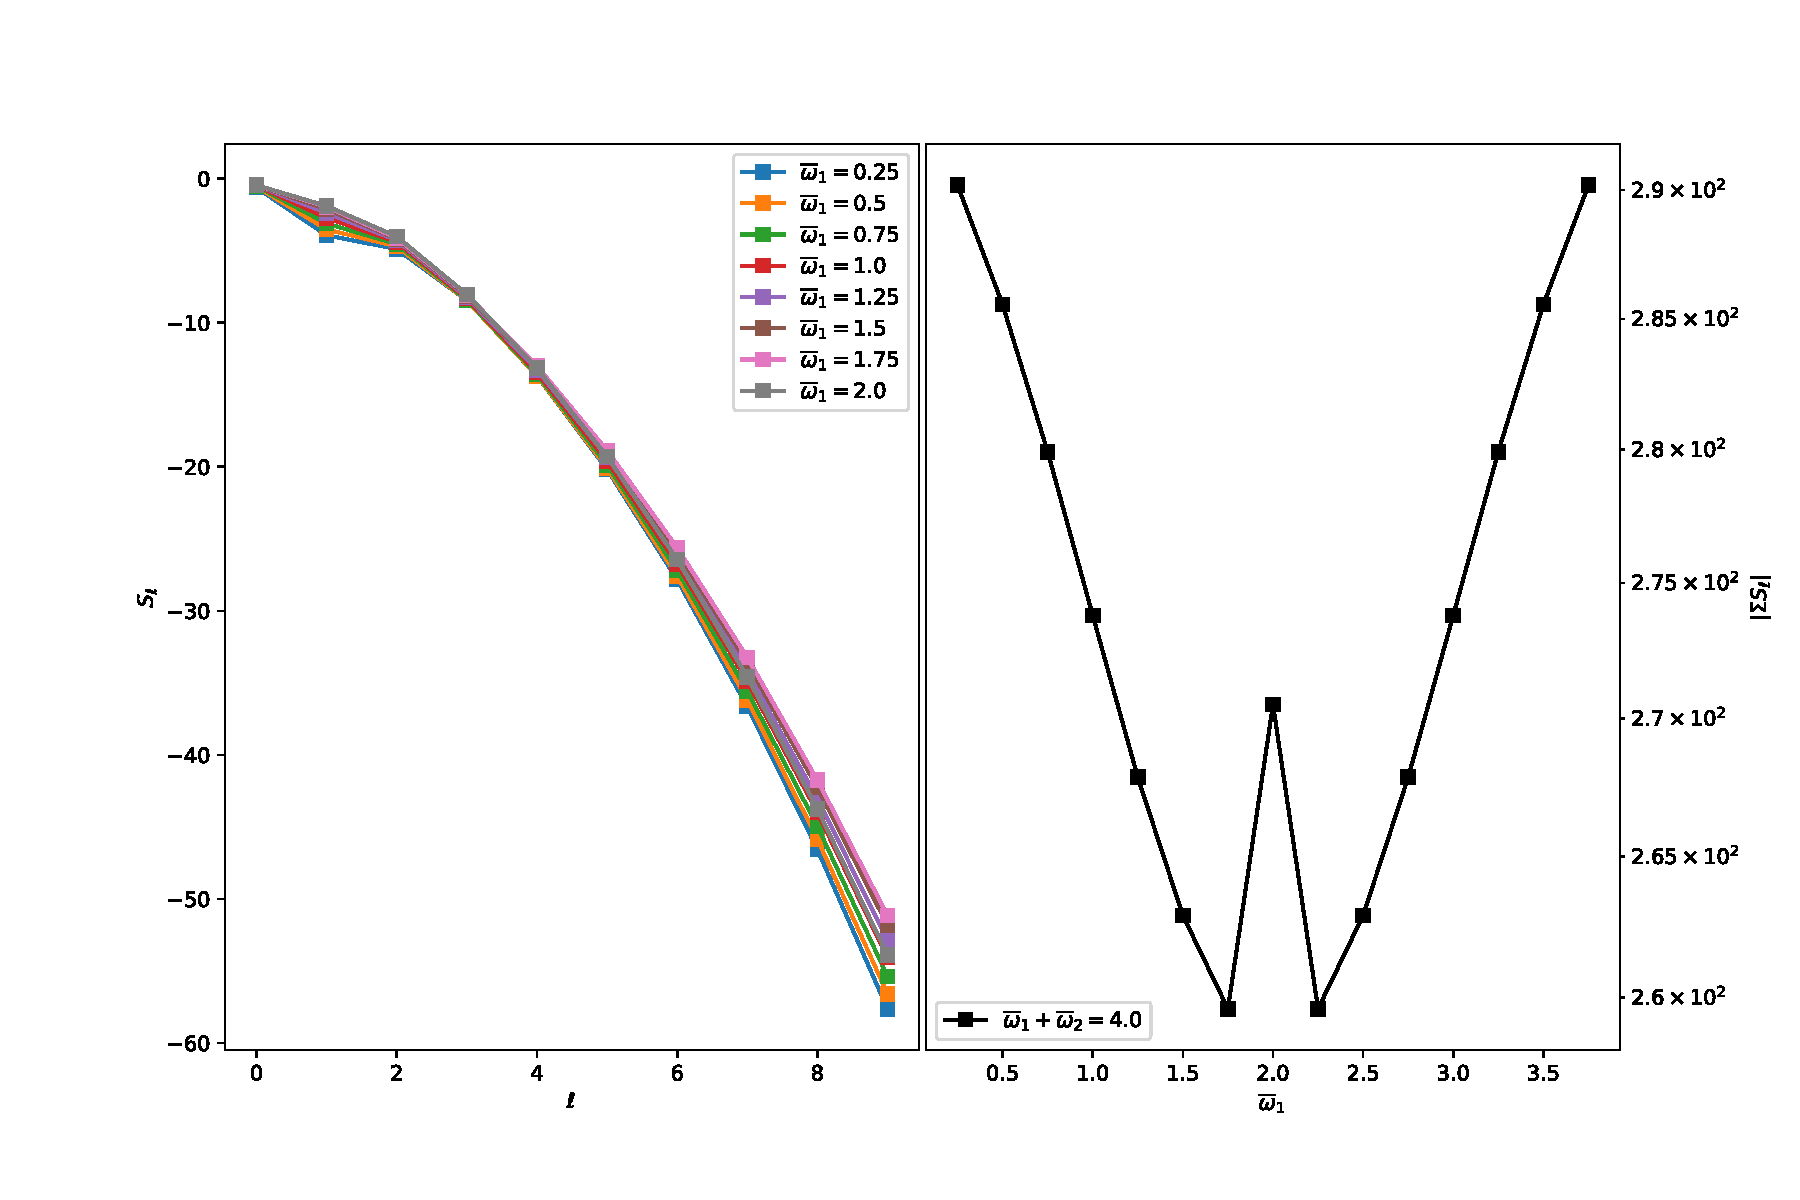
\includegraphics[width=\textwidth]{./figures/NNAddToInteger_source_n2_m-4_0}
\caption{{\it Left}: Source term values for a tachyonic scalar with $m^2 = -4.0$ when the frequencies of non-normalizable modes sum to $4.0$. {\it Right}: The absolute value of the sum of the source terms for each choice of $\oone$, $\otwo$.}
\label{fig:atoi_all_m-4_0}
\end{figure}

\begin{figure}[h!]
\centering
	\begin{subfigure}[b]{0.75\textwidth}
		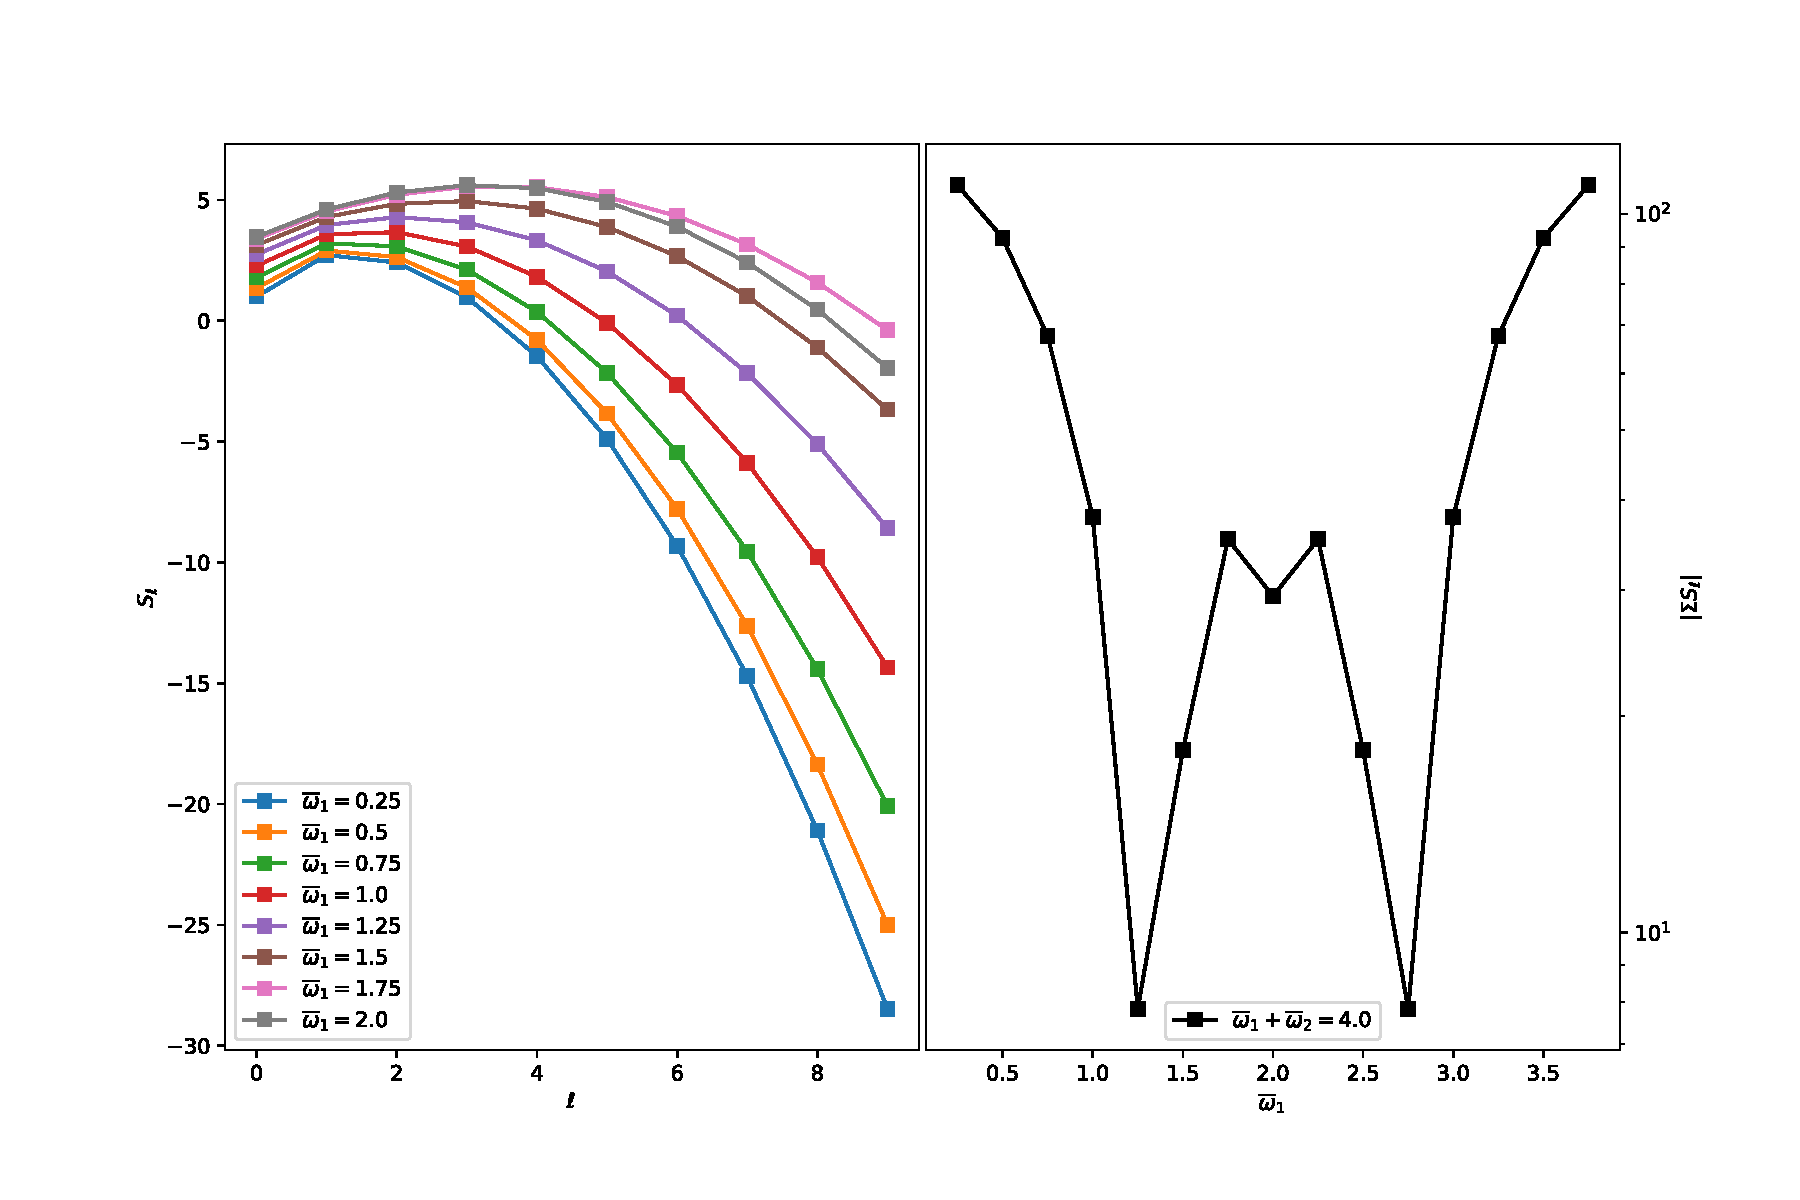
\includegraphics[width=\textwidth]{./figures/NNAddToInteger_source_n2_m0_0}
		\label{fig:atoi_all_n2_m0}
	\end{subfigure}
	\vspace{-0.25in}
	\begin{subfigure}[b]{0.75\textwidth}
		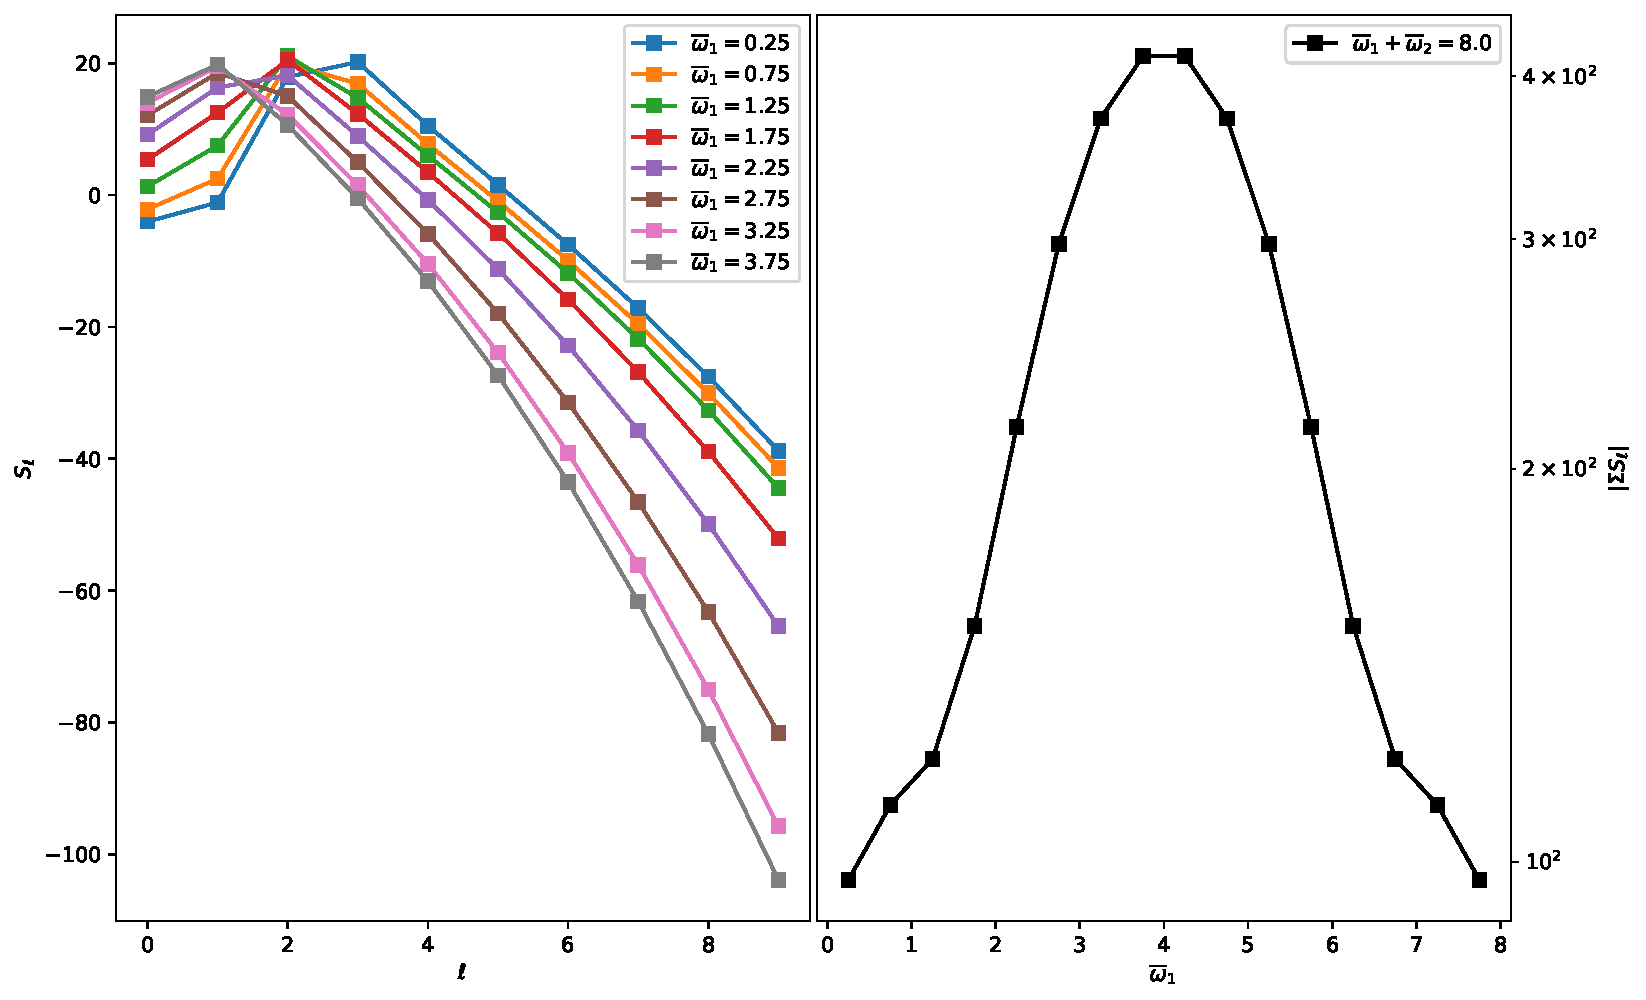
\includegraphics[width=\textwidth]{./figures/NNAddToInteger_source_n4_m0_0}
		\label{fig:atoi_all_n4_m0}
	\end{subfigure}
	\caption{{\it Above:} The value of \eqref{add to integer} as a function of $\ell$ for a massless scalar with values of $\oone$ and $\otwo$ chosen so that $\oone + \otwo = 4$. {\it Below:} The same plot but with values chosen to satisfy $\oone + \otwo = 8$.}
	\label{fig:atoi_all_m0_0compare}
\end{figure}

\subsection{Integer Plus $\chi$}

This is a case where the non-normalizable frequencies are non-integer, but differ from integer values by a specific amount. In analogue to the case where all modes are normalizable, we consider setting any two of the non-normalizable frequencies to
\begin{align}
\ogam = 2\gamma + \chi \, ,
\end{align}
where $m^2$ is \emph{not} chosen to be a special value\footnote{By tuning the value of the mass so that $\chi$ is an integer, additional resonant terms are possible; however, this scenario is addressed in \S\!~\ref{ssec: add to integer}. Furthermore, we do not consider the case when the Breitenlohmer-Freeman bound is saturated. This would place further restrictions on the allowed values of the indices in certain terms since the difference between the frequencies of normalizable and non-normalizable modes could then be zero.}, i.e. $\chi \notin \mathbb{Z}^*$, and $\gamma$ is an integer (greek letters are chosen to differentiate between normalizable modes with integer frequencies that use roman letters). For this choice of non-normalizable frequencies, there are no resonant contributions from the all-plus channel; only when either $\oi + \ogam = \obet - \ol$, or $\oi + \ogam = \obet + \ol$ with $i + \gamma \geq \ell$, are resonant terms present.

\subsubsection{$\oi + \ogam = \obet - \ol$}

This channel contributes secular terms of the form
\begin{align}
S_\ell &= \sum_{i \neq \ell} \sum_{\gamma \neq \beta} \overline{S}_{i (i + \gamma + \ell) \gamma \ell} \cos \left( \theta_i - \theta_{(i + \gamma + \ell)} + \theta_\gamma \right) + \sum_\beta \overline{R}_{\ell \beta} \cos \left(\theta_\ell + \theta_\beta - \theta_\beta \right) 
\end{align}
where 
\begin{align}
\overline{S}_{i \beta\gamma\ell} &= - \frac{1}{4} Z^+_{\beta\gamma i \ell} \left( \frac{\oi}{\oi + \ol}\right) + \frac{1}{4} Z^{-}_{i\gamma\beta\ell} \left(  \frac{\obet}{\ol - \obet}  \right) + \frac{1}{4} Z^+_{i\beta\gamma\ell} \left( \frac{\ogam}{\ol + \ogam} \right) \nonumber \\
%
& + \frac{1}{4} \bigg[ \frac{1}{\obet - \ogam} \left( \ogam H_{\beta\gamma i \ell} - \obet H_{\gamma \beta i \ell} - 2\oi^2 \left( \ogam X_{\beta\gamma i \ell} - \obet X_{\gamma \beta i \ell} \right) \right)\nonumber \\
%
& \quad - \frac{1}{\oi + \ogam} \left( \oi H_{\gamma i \beta \ell}  + \ogam H_{i \gamma\beta\ell} - 2\obet^2 \left( \oi X_{\gamma i \beta\ell} + \ogam X_{i \gamma\beta \ell} \right) \right) \nonumber \\
%
& \quad + \frac{1}{\oi - \obet} \left( \obet H_{i\beta\gamma\ell} - \oi H_{\beta i \gamma \ell} - 2 \ogam^2 \left( \obet X_{i \beta \gamma \ell} - \oi X_{\beta i \gamma \ell} \right) \right) \nonumber \\
%
& \quad -2 \obet \ogam X_{i\beta\gamma\ell} -2 \oi\obet X_{\gamma i \beta\ell} + 2 \oi\ogam X_{\beta i \gamma\ell} \bigg]
\end{align}
and
\begin{align}
\overline{R}_{\ell \beta} &= \frac{1}{4}  \bigg[ Z^{-}_{\ell \beta \beta \ell} \left( \frac{\obet}{\ol + \obet} \right) +  Z^+_{\ell \beta \beta \ell} \left(\frac{\obet}{\ol - \obet} \right) + 2 H_{\ell\beta\beta\ell} \left( \frac{\obet^2}{\ol^2 - \obet^2} \right)  \nonumber \\
%
& - 2H_{\beta \ell\beta\ell} \left( \frac{\ol^2}{\ol^2 - \obet^2} \right) + 4 X_{\beta\ell\beta\ell} \left( \frac{\ol^2 \obet^2}{\ol^2 - \obet^2} \right)  - 4 X_{\beta\ell\beta\ell} \left( \frac{\obet^4}{\ol^2 - \obet^2} \right)  \nonumber \\
%
&  - 2\obet^2 X_{\ell\beta\beta\ell} + 4 \ol^2 X_{\beta\ell\beta\ell} + 4 \ol^2 \tilde{Z}^+_{\beta\beta\ell} - 2H_{\beta\beta\ell\ell}  - 8 \obet^2 \ol^2 P_{\ell\ell\beta} - 4 \obet^2 M_{\ell\ell\beta} \bigg]
\end{align}

\subsubsection{$\oi + \ogam = \obet + \ol$}
This channel contributes secular terms of the form
\begin{align}
S_\ell = \underbrace{\sum_{i \neq \ell} \sum_{\gamma \neq \beta}}_{i + \gamma \geq \ell} \overline{S}_{i (i + \gamma - \ell) \gamma \ell} \cos \left( \theta_i - \theta_{(i + \gamma - \ell)} + \theta_\gamma \right) + \sum_\beta \overline{R}_{\ell \beta} \cos \left( \theta_\ell + \theta_\beta - \theta_\beta \right)
\end{align}
where
\begin{align}
\overline{S}_{i\beta\gamma\ell} &= \frac{1}{4} Z^-_{i\gamma\beta\ell} \left( \frac{\obet}{\ol + \obet}\right)  + \frac{1}{4} Z^+_{i\beta\gamma\ell} \left( \frac{\ogam}{\ol - \ogam}\right)  - \frac{1}{4}Z^+_{\beta\gamma i \ell} \left( \frac{\oi}{\oi - \ol} \right) \nonumber \\
%
& + \frac{1}{4}\bigg[  \frac{1}{\obet - \ogam} \left( \ogam H_{\beta\gamma i \ell} - \obet H_{\gamma\beta i \ell} - 2\oi^2 \left( \ogam X_{\beta\gamma i \ell} - \obet X_{\gamma\beta i \ell} \right) \right) \nonumber \\
%
& \quad + \frac{1}{\oi - \obet} \left( \obet H_{i\beta\gamma\ell} - \oi H_{\beta i \gamma\ell}  -2 \ogam^2 \left( \obet X_{i\beta\gamma\ell} - \oi X_{\beta i \gamma\ell} \right) \right) \nonumber \\
%
& \quad + \frac{1}{\oi - \ogam} \left( \oi H_{\gamma i \beta\ell} - \ogam H_{i\gamma\beta\ell} - 2\obet^2 \left( \oi X_{\gamma i \beta\ell} - \ogam X_{i\gamma\beta\ell} \right) \right) \nonumber \\
%
& \quad - 2 \oi\obet X_{\gamma i \beta\ell} - 2 \obet\ogam X_{i\beta\gamma\ell} + 2\oi\ogam X_{\beta\gamma i\ell}\bigg]
\end{align}
and
\begin{align}
\overline{R}_{\ell \alpha} &= \frac{1}{4} \bigg[ Z^-_{\ell\beta\beta\ell} \left( \frac{\obet}{\ol + \obet} \right) + Z^+_{\ell\beta\beta\ell} \left( \frac{\obet}{\ol - \obet} \right) + 2 H_{\ell\beta\beta\ell} \left( \frac{\obet^2}{\ol^2 - \obet^2} \right) \nonumber \\
%
& - 2 H_{\beta\ell\beta\ell} \left( \frac{\ol^2}{\ol^2 - \obet^2} \right) - 4 X_{\ell\beta\beta\ell} \left( \frac{\obet^4}{\ol^2 - \obet^2} \right) + 4 X_{\beta\ell\beta\ell} \left( \frac{\ol^2 \obet^2}{\ol^2 - \obet^2} \right) \nonumber \\
%
& - 2 \obet^2 X_{\ell \beta\beta \ell} + 4\ol^2 \tilde{Z}^+_{\beta\beta\ell} + 4 \ol^2 X_{\beta\beta\ell\ell} - 2 H_{\beta\beta\ell\ell} - 8 \obet^2 \ol^2 P_{\ell\ell\beta} - 4 \obet^2 M_{\ell\ell\beta} \bigg] \, .
\end{align}

%%%%%%%%%%%%%%%%%%%%%%%%%%%%%%%%%%%%%%%%%
%%%%%%%%%%%%%%%%%%%%%%%%%%%%%%%%%%%%%%%%%

\section{QP Equations}

%%%%%%%%%%%%%%%%%%%%%%%%%%%%%%%%%%%%%%%%%
%%%%%%%%%%%%%%%%%%%%%%%%%%%%%%%%%%%%%%%%%

\section{Discussion}

%%%%%%%%%%%%%%%%%%%%%%%%%%%%%%%%%%%%%%%%%
%%%%%%%%%%%%%%%%%%%%%%%%%%%%%%%%%%%%%%%%%

%\acknowledgments

%%%%%%%%%%%%%%%%%%%%%%%%%%%%%%%%%%%%%%%%%
%%%%%%%%%%%%%%%%%%%%%%%%%%%%%%%%%%%%%%%%%

\appendix
\section{Derivation of Source Terms For Massive Scalars}
\label{source term derivation}
The derivation of the source terms for massive scalars closely follows the massless case, particularly if one chooses not to write out the explicit mass dependence as was done in \cite{1810.04753}. However, since we have chosen to write our equations in a slightly different way -- and in a different gauge -- than previous authors, one may find it instructive to see the differences in the derivations. Below we have included the intermediate steps involved in deriving the third-order source term $S_\ell$.

Projecting each of the terms individually onto the eigenbasis $\{ e_\ell \}$:
\begin{align}
\langle \delta_2 \ddot \phi_1, e_\ell \rangle &= - \sum_{i = 0}^\infty \sum_{\substack{j=0 \\ k \neq \ell}}^\infty \sum_{k=0}^\infty \frac{\ok^2 c_k}{\ol^2 - \ok^2} \left[\dot c_i \dot c_j \left(X_{k\ell ij} - X_{\ell k i j} \right) + c_i c_j \left( Y_{ij\ell k} - Y_{ijk\ell} \right) \right] \nonumber \\
& \qquad  - \sum_{i=0}^\infty \sum_{j=0}^\infty \ol^2 c_\ell \left[ \dot c_i \dot c_j P_{ij\ell} + c_i c_j B_{i j \ell} \right] \, , \\
%
\langle A_2 \ddot \phi_1, e_\ell \rangle &= 2 \sum_{i = 0}^\infty \sum_{\substack{j=0 \\ i \neq j}}^\infty \sum_{k=0}^\infty \frac{\ok^2 c_k}{\oj^2 - \oi^2} X_{ijk \ell} \left( \dot c_i \dot c_j + \oj^2 c_i c_j \right) \nonumber \\
& \qquad + \sum_{i = 0}^\infty \sum_{j = 0}^\infty \oj^2 c_j \left( \mathbb C_i P_{j \ell i} + c_i^2 X_{ii j \ell} \right) \, , \\
%
\langle \dot \delta_2 \dot \phi_1 , e_\ell \rangle &= \sum_{i = 0}^\infty \sum_{\substack{j=0 \\ k \neq \ell}}^\infty \sum_{k=0}^\infty \frac{\dot c_k}{\ol^2 - \ok^2} \left[ \p_t \left( \dot c_i \dot c_j \right) \left( X_{k\ell ij} - X_{\ell k i j} \right) + \p_t (c_i c_j) \left(Y_{ij\ell k} - Y_{ijk\ell}\right) \right] \nonumber \\
& \qquad+ \sum_{i=0}^\infty \sum_{j=0}^\infty \dot c_\ell \left[ \p_t \left( \dot c_i \dot c_j \right) P_{ij\ell} + \p_t (c_i c_j) B_{ij\ell} \right] \, , \\
%
\langle \dot A_2 \dot \phi_1, e_\ell \rangle &= -2 \sum_{i=0}^\infty \sum_{j=0}^\infty \sum_{k=0}^\infty  \dot c_k \dot c_j c_i X_{ijk\ell} \, , \\
%
\langle \left( A_2' - \delta_2' \right) \phi_1', e_\ell \rangle &= - 2 \sum_{i = 0}^\infty \sum_{\substack{j=0 \\ i \neq j}}^\infty \sum_{k=0}^\infty \frac{c_k (\dot c_i \dot c_j + \oj^2 c_i c_j)}{\oj^2 -\oi^2} H_{ijk\ell} -m^2 \sum_{i=0}^\infty \sum _{j=0}^\infty \sum_{k=0}^\infty c_i c_j c_k V_{ijk\ell} \nonumber \\
%
& \qquad - \sum_{i=0}^\infty \sum_{j=0}^\infty c_j \left[ c_i^2 H_{iij\ell} + \mathbb C_i M_{j \ell i} \right] \, , \\
%
\langle A_2 \phi_1 \sec^2 x, e_\ell \rangle &= - 2\sum_{i = 0}^\infty \sum_{\substack{j=0 \\ i \neq j}}^\infty \sum_{k=0}^\infty \frac{c_k (\dot c_i \dot c_j + \oj^2 c_i c_j )}{\oj^2 - \oi^2} V_{jki\ell} \nonumber \\
& \qquad - \sum_{i=0}^\infty \sum_{j=0}^\infty c_j \left( c_i^2 V_{jii\ell} + \mathbb C_i Q_{j\ell i} \right) .
\end{align}

Where the forms of X, Y, V, H, B, M, P, and Q are given by
\begin{align}
X_{ijk\ell} &= \int^{\pi/2}_0 dx \, \mu^2 \nu e'_i e_j e_k e_\ell \\
Y_{ijk\ell} &= \int^{\pi/2}_0 dx \, \mu^2 \nu e'_i e'_j e_k e'_\ell \\
V_{ijk\ell} &= \int^{\pi/2}_0 dx \, \mu^2 \nu e_i e_j e'_k e_\ell \sec^2 x \\
H_{ijk\ell} &= \int^{\pi/2}_0 dx \, \mu^2 \nu' e'_i e_j e'_k e_\ell \\
B_{ij\ell} &= \int^{\pi/2}_0 dx \, \mu \nu e'_i e'_j \int^x_0 dy \, \mu e^2_\ell \\
M_{ij\ell} &= \int^{\pi/2}_0 dx \, \mu \nu' e'_i e_j \int^x_o dy \, \mu e_\ell^2 \\
P_{ij\ell} &= \int^{\pi/2}_0 dx \, \mu \nu e_i e_j \int^x_0 dy \, \mu e^2_\ell \\
Q_{ij\ell} &= \int^{\pi/2}_0 dx \, \mu \nu e_i e_j \sec^2 x \int^x_0 dy \, \mu e^2_\ell
\end{align}

Collecting terms together gives the expression for $S_\ell = \langle S, e_\ell \rangle$:
\begin{align}
S_\ell &= \sum_{\substack{i, j, k \\ k \neq \ell}}^\infty \frac{1}{\ol^2 - \ok^2} \Big[ F_k(\dot c_i \dot c_j) \left(X_{k\ell i j} - X_{\ell k i j} \right) + F_k(c_i c_j) \left(Y_{ij\ell k} - Y_{ijk\ell} \right) \Big] \nonumber \\
%
& \quad +2 \sum_{\substack{i,j,k \\ i \neq j}}^\infty \frac{c_k D_{ij}}{\oj^2 - \oi^2} \Big[  2\ok^2 X_{ijk\ell} - H_{ijk\ell} -m^2 V_{jki\ell} \Big] - \sum_{i,j,k}^\infty c_i \Big[ 2 \dot c_j \dot c_k X_{ijk\ell} + m^2 c_j c_k V_{ijk\ell} \Big] \nonumber \\ 
%
& \quad + \sum_{i,j}^\infty \Big[ F_\ell (\dot c_i \dot c_j) P_{ij\ell} + F_\ell (c_i c_j) B_{ij\ell} + 2\oj^2 c_j \left( c_i^2 X_{iij\ell} + \mathbb C_i P_{j\ell i} \right) \nonumber \\
%
& \qquad - c_j \left( c^2_i (H_{iij\ell} + m^2 V_{jii\ell} ) + \mathbb C_i (M_{j\ell i} + m^2 Q_{j\ell i}) \right) \Big] \, ,
\end{align}
where $F_k(z) = \dot c_k \dot z - 2\ok^2 c_k z$, $D_{ij} = \dot c_i \dot c_j + \omega^2_j c_i c_j$, and $\mathbb C_i = \dot c_i^2 + \oi^2 c_i^2$.

To simplify the above expression, we have defined
\begin{align}
Z^{\pm}_{ijk\ell} = \oi \oj \left( X_{k\ell ij} - X_{\ell kij} \right) \pm \left( Y_{ij\ell k} - Y_{ijk\ell} \right) \quad \text{and} \quad \tilde Z^{\pm}_{ij\ell} = \oi \oj P_{ij\ell} \pm B_{ij\ell} \, .
\end{align}

Using integration by parts to remove the derivative from $\nu$ in the definitions of $H_{ijk\ell}$ and $M_{ij\ell}$, we can show that
\begin{align}
H_{ijk\ell} &= \oi^2 X_{kij\ell} + \ok^2 X_{ijk\ell} - Y_{ij\ell k}  - Y_{\ell kji}   - m^2 V_{kji\ell} -m^2 V_{ijk\ell} \\
M_{ij\ell} &= \oi^2 P_{ij\ell} - B_{ij\ell} -m^2 Q_{ij\ell}
\end{align}

\section{Two Non-normalizable Modes with Equal Frequencies}
\label{more 2NN}

Consider activating two non-normalizable modes at the same general frequency, $\ob$. In such a case, any two of the summed indices may represent a non-normalizable frequency. These non-normalizable modes may have frequencies that happen to satisfy $\ob = \ol$ numerically; this does not change the fact that their basis functions are given by \eqref{general basis}. With this is mind, the same time averaging procedure restricts the presence of resonant contributions to those that satisfy \eqref{gen res}. Since the basis onto which we are projecting is normalizable, we know that $\ol = 2\ell + \Delta^+$, which means there are four cases in which resonance may occur.

Discuss difference resonances for special cases of $\ob$ beyond the arbitrary value condition covered in the main portion. 

In addition to the case of arbitrary values of $\ob$, the following resonances contribute to the source term $S_\ell$ via
\begin{align}
S_\ell &= a_\ell A^2_{\ob} \left[ \overline{R}^{(1)}_{i \ob} \cos \left( \theta_i - 2\ob t \right) + \overline{R}^{(2)}_{i \ob} \cos \left( \theta_i + 2\ob t \right) + \overline{R}^{(3)}_{i \ob} \cos \left( 2\ob t - \theta_i \right) \right] \Big|_{i = \ell}
\end{align}
under their respective conditions on the value of $\ob$:
\begin{align}
\label{gen NN res}
\overline{R}^{(1)}_{\ell \ob}: \quad \omega_I &= \ol + 2\ob \quad I \in \{i,j,k\} \; \forall \; \ob \in \mathbb{Z}^* \\
\overline{R}^{(2)}_{\ell \ob}: \quad \omega_I &= \ol - 2\ob \quad I \in \{i,j,k\} \; \forall \; \ob \in \mathbb{Z}^* \; \text{such that } \ell \geq \ob \\
\overline{R}^{(3)}_{\ell \ob}: \quad \omega_I &= 2\ob - \ol \quad I \in \{i,j,k\} \; \forall \; \ob \in \mathbb{Z}^* \; \text{such that } \ell \leq \ob
\end{align}

When $\ob \in \mathbb{Z}^*  \leq \ell$, resonance is at $\oi = \ol - 2\ob$ with 
\begin{align}
\overline{R}^{(1)}_{i \ob} &= - \frac{1}{12} \left(1 - \delta(\ol - \ob) \right) Z^-_{i \ob \ob \ell} \left(\frac{\ob}{\ol - \ob} \right) \nonumber \\
%
& \quad - \frac{1}{12} (1 - \delta(\oi - \ob) \Big \{ \left( \frac{\ob}{\oi + \ob} \right) \left(H_{i\ob\ob\ell} + m^2 V_{\ob\ob i \ell} - 2\ob^2 X_{i\ob\ob\ell} \right) + \nonumber \\
%
& \quad + \left( \frac{\ol - 2\ob}{\oi + \ob} \right) \left( H_{\ob i \ob \ell} + m^2 V_{i \ob \ob \ell} - 2 \ob^2 X_{\ob i \ob \ell} \right) \Big] \nonumber \\
%
& \quad - \frac{(\ol - 2\ob)}{48\ob} Z^-_{\ob\ob i \ell} + \frac{1}{12} \ob^2 X_{i \ob \ob \ell} + \frac{\ob (\ol - 2\ob)}{12} X_{\ob\ob i \ell} - \frac{m^2}{12} V_{i\ob\ob\ell} - \frac{m^2}{24} V_{\ob\ob i \ell} \, .
\end{align}

When $\ob \in \mathbb{Z}^*$ and $\ob \geq \ob$:
\begin{align}
\overline{R}^{(2)}_{i \ob} &= \, .
\end{align}

When $\ob \in \mathbb{Z}^*$ and $\ob \leq \ob$:
\begin{align}
\overline{R}^{(3)}_{i\ob} &= \, .
\end{align}



%%%%%%%%%%%%%%%%%%%%%%%%%%%%%%%%%%%%%%%%%
%%%%%%%%%%%%%%%%%%%%%%%%%%%%%%%%%%%%%%%%%

\bibliographystyle{JHEP}
\bibliography{DrivenTTF}

%%%%%%%%%%%%%%%%%%%%%%%%%%%%%%%%%%%%%%%%%
%%%%%%%%%%%%%%%%%%%%%%%%%%%%%%%%%%%%%%%%%

\end{document}

%%%%%%%%%%%%%%%%%%%%%%%%%%%%%%%%%%%%%%%%%
%%%%%%%%%%%%%%%%%%%%%%%%%%%%%%%%%%%%%%%%%


\begin{figure}
\centering
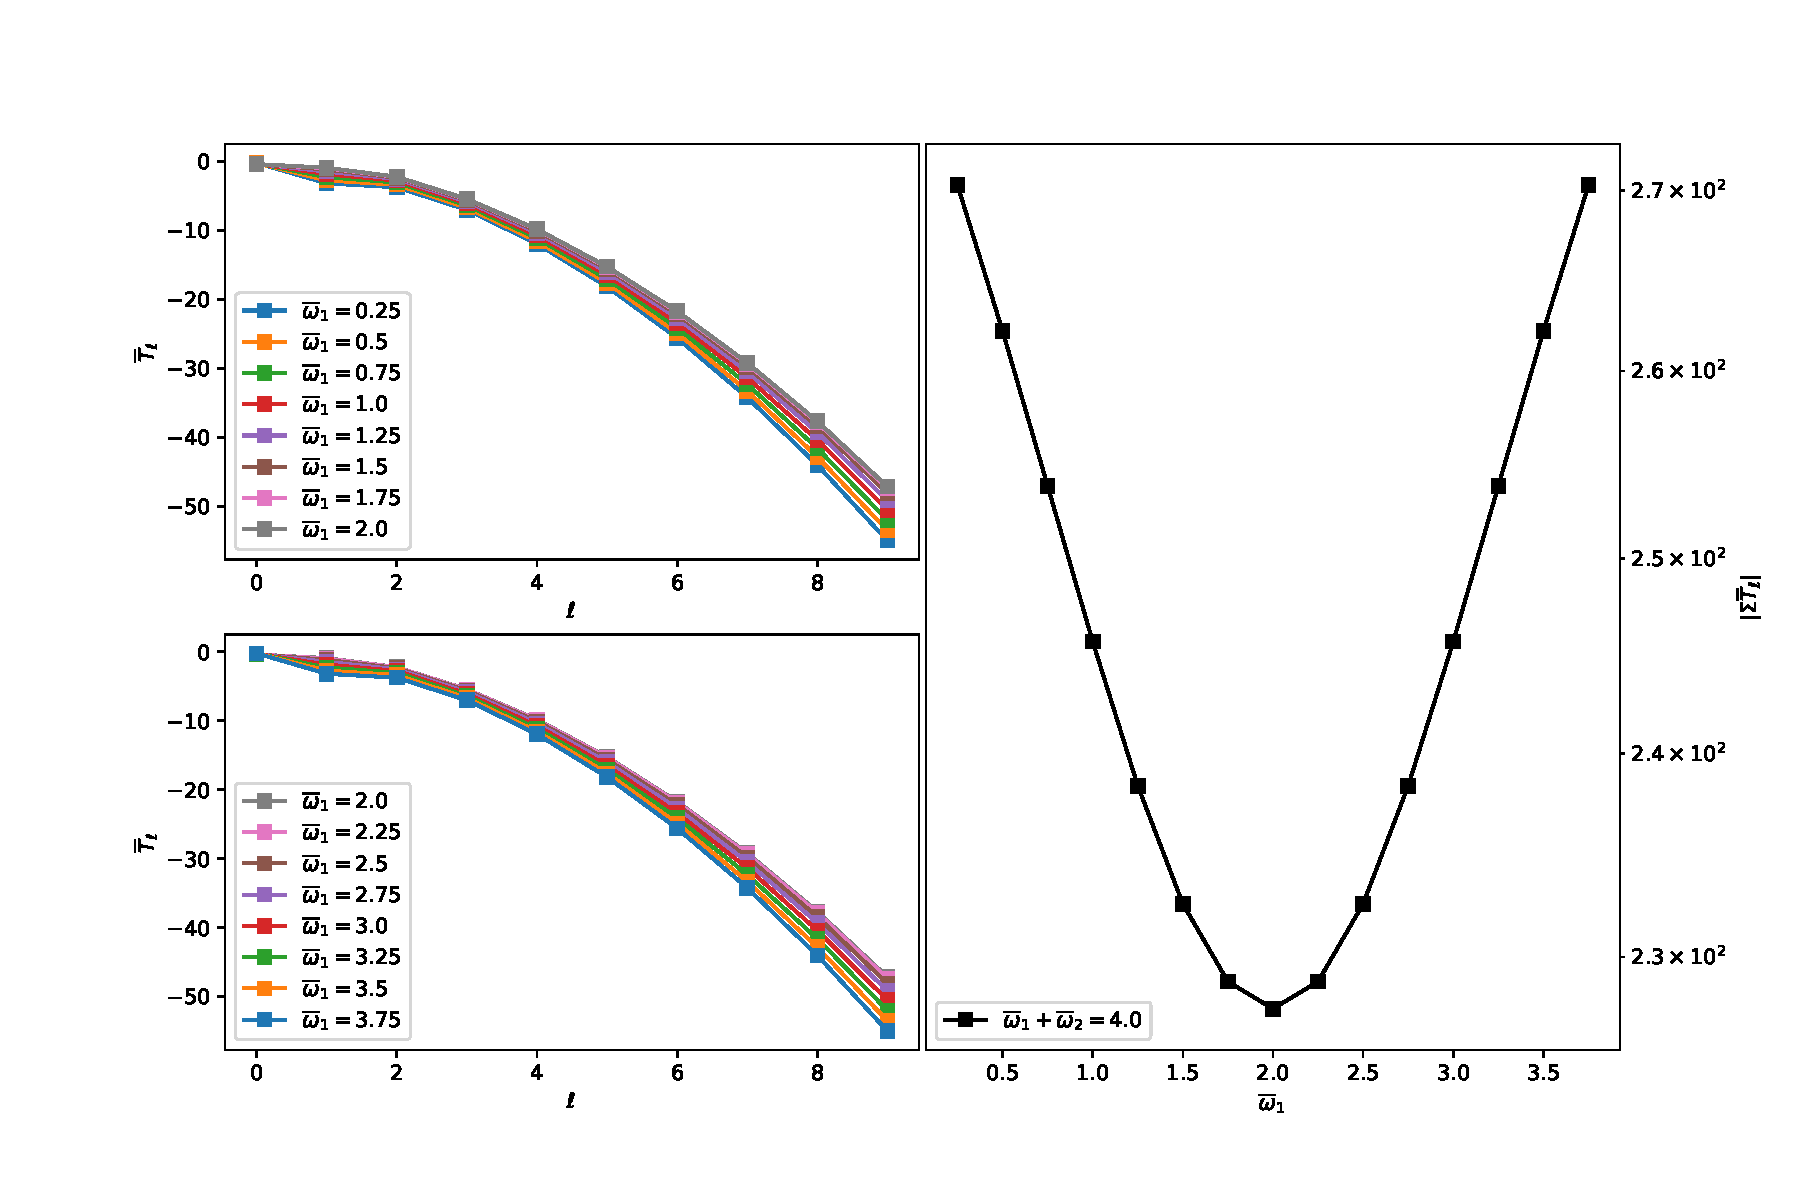
\includegraphics[width=\textwidth]{./figures/NN_equalfreq_tchannel_n2_m-4_0}
\caption{{\it Left, above}: . {\it Left, below}: .{\it Right}: $m^2 = -4.0$.}
\label{fig:atoi_t_m-4_0}
\end{figure}

\begin{figure}
\centering
	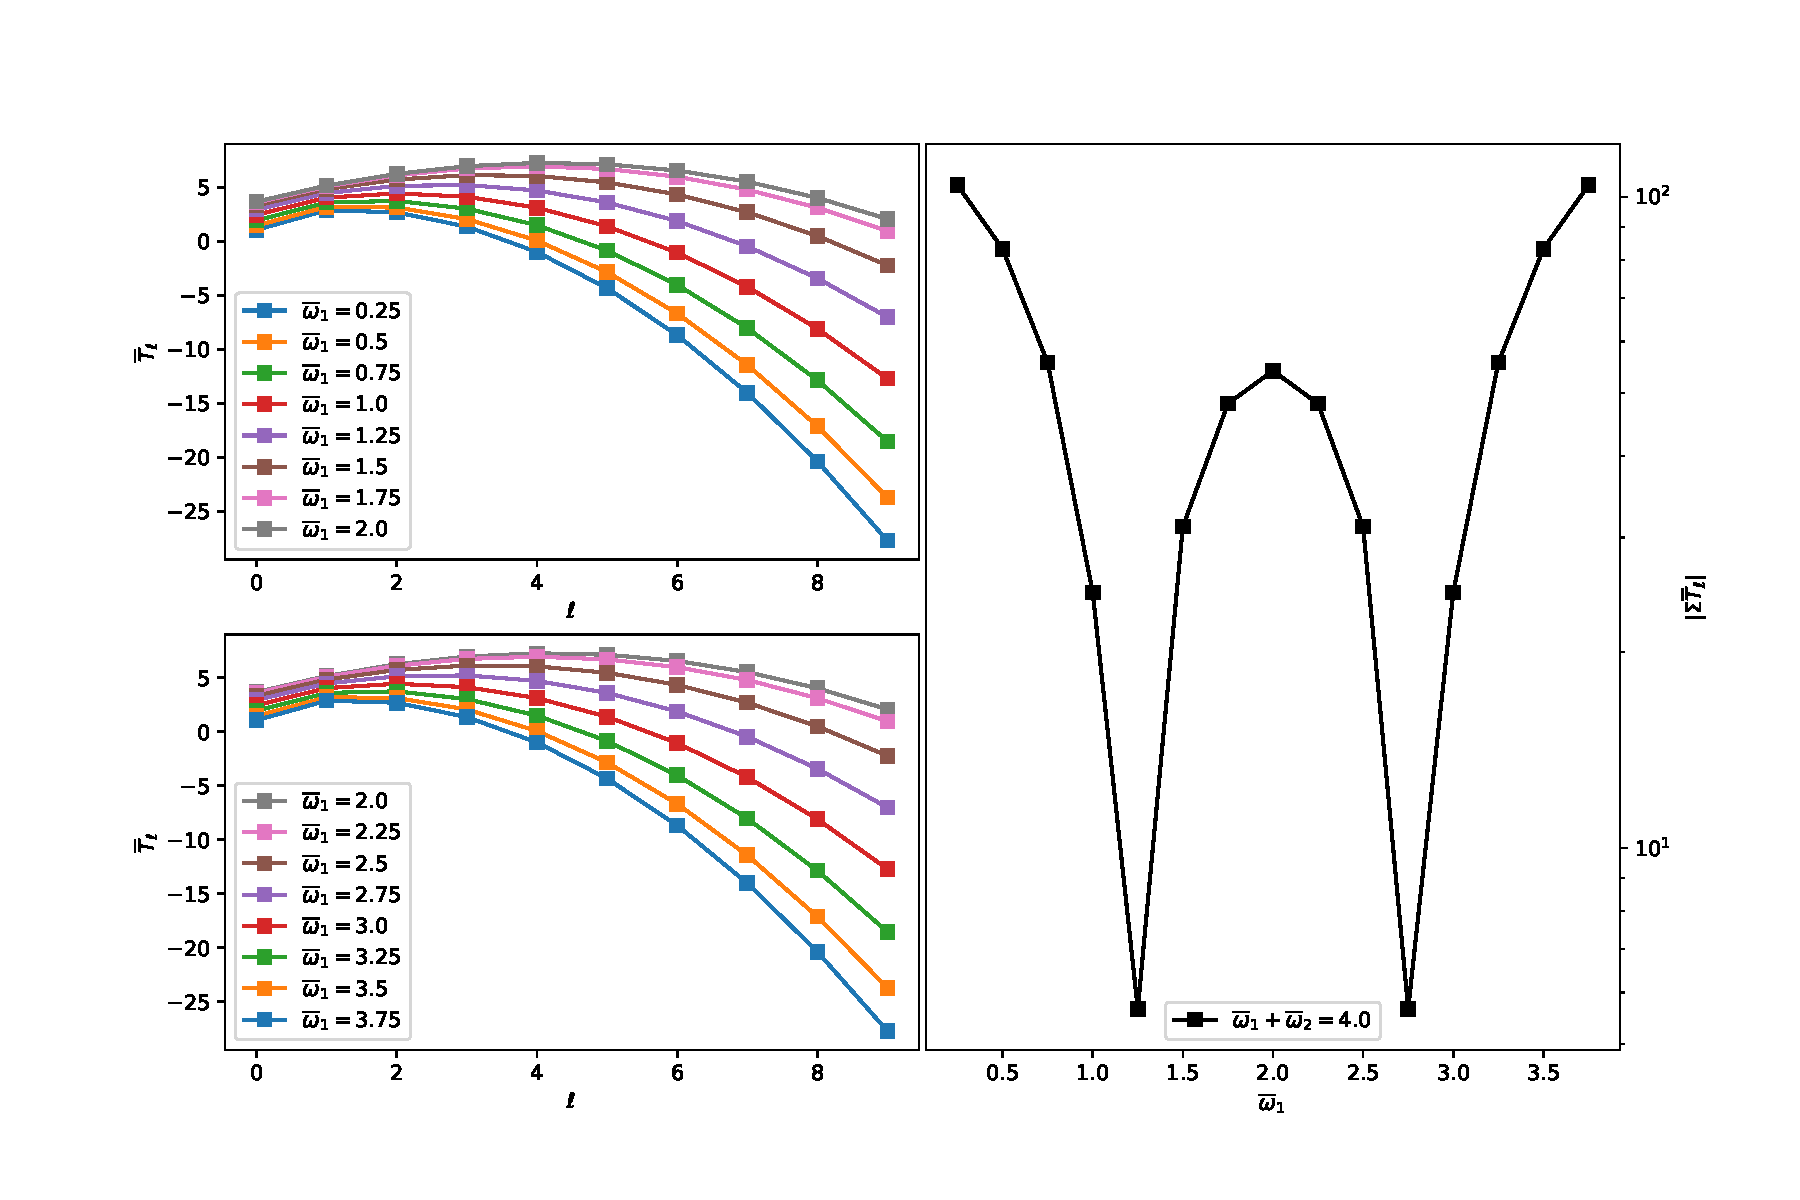
\includegraphics[width=\textwidth]{./figures/NN_equalfreq_tchannel_n2_m0_0}
	\caption{$\overline{T}$ for $m^2 = 0$.}
\end{figure}

\begin{figure}
\centering
	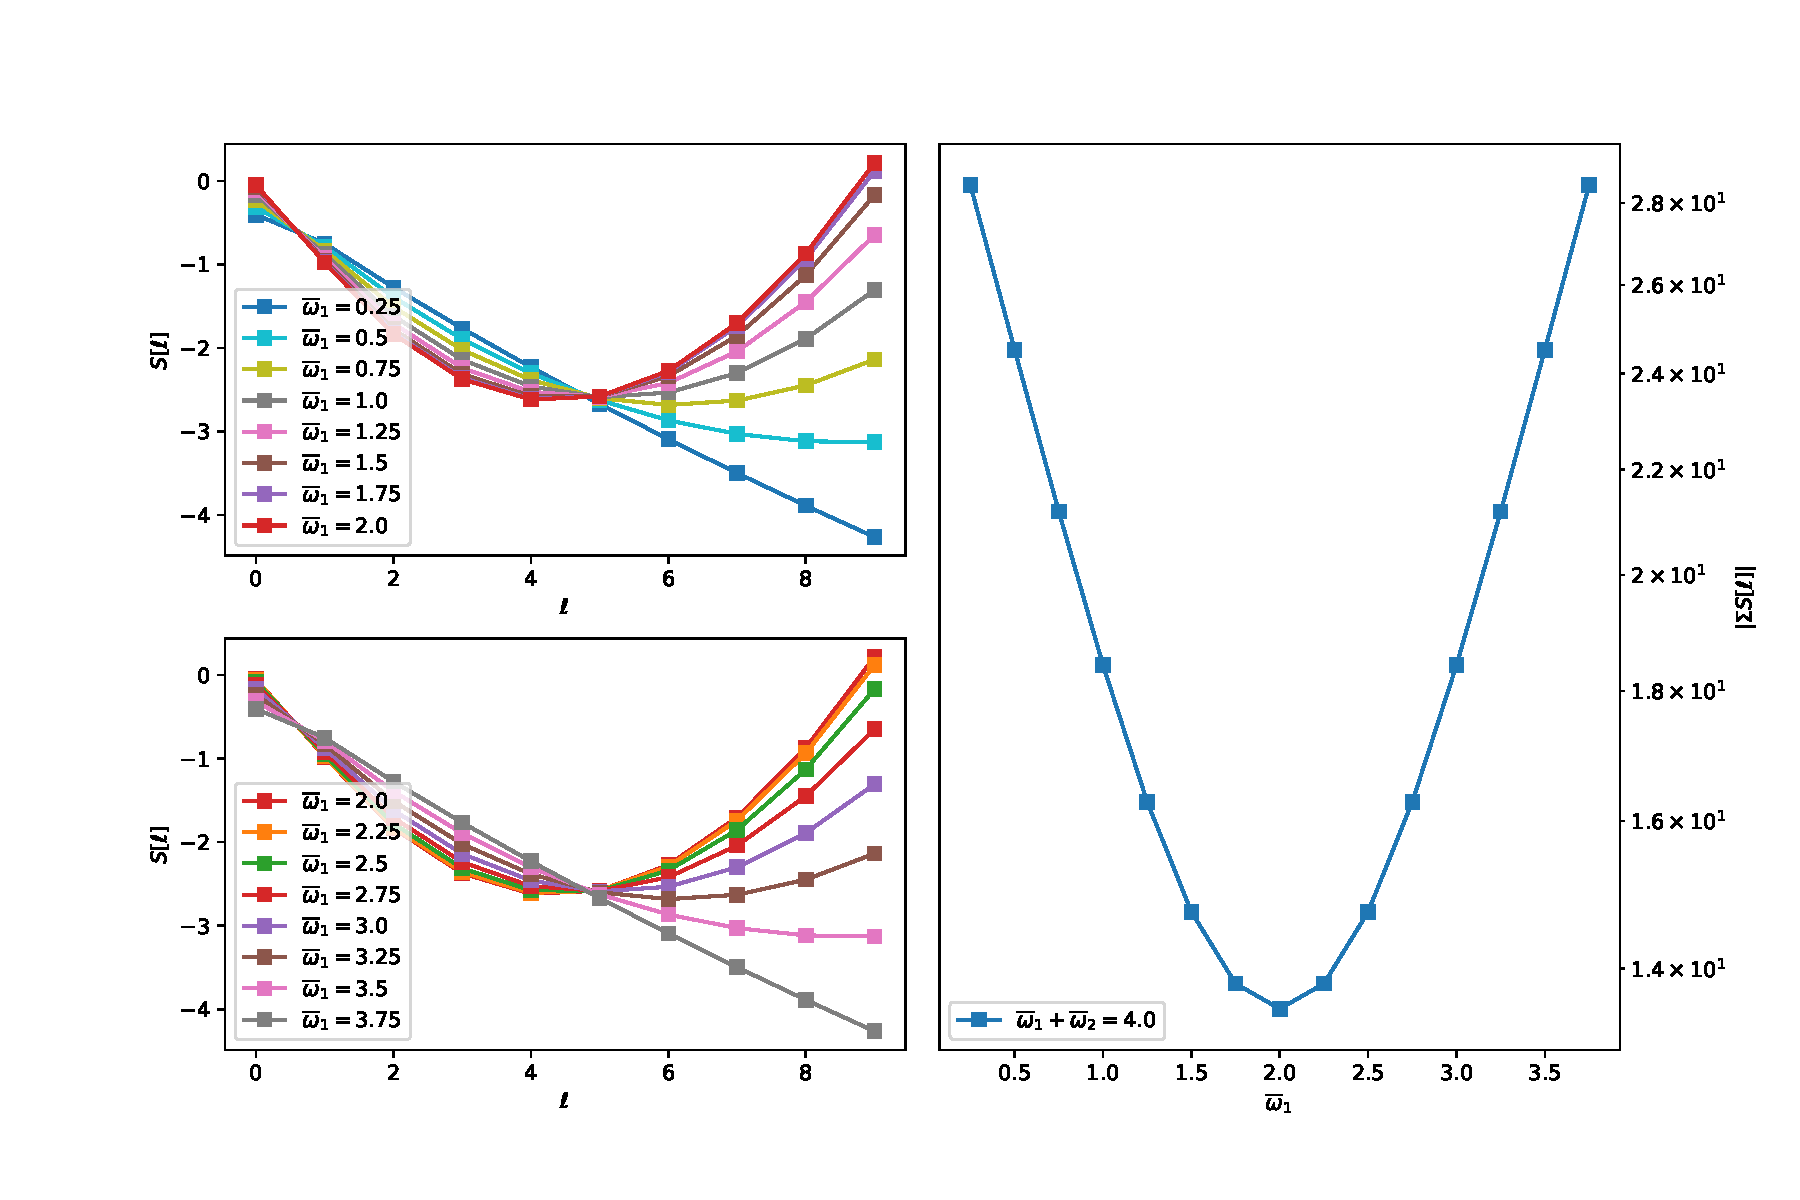
\includegraphics[width=\textwidth]{./figures/NN_equalfreq_pmchannel_n2_m-4_0}
	\caption{{\it Left, above}: Individual values of $\overline{R}^{(+-)}_{(\ell - n)12\ell}$ for $m^2 = -4.0$ as a function of $\ell$ for $\oone + \otwo = 2n$ with $n = 4$ when $\oone \leq n$. {\it Left, below}: The same function, but for $\oone \geq n$; note the symmetry in values as $\oone \leftrightarrow \otwo$. {\it Right}: The absolute value of the sum of the $(+-)$ source terms for choices of $\oone$.}
	\label{fig:atoi_pm_m-4_0}
\end{figure}

\begin{figure}
\centering
	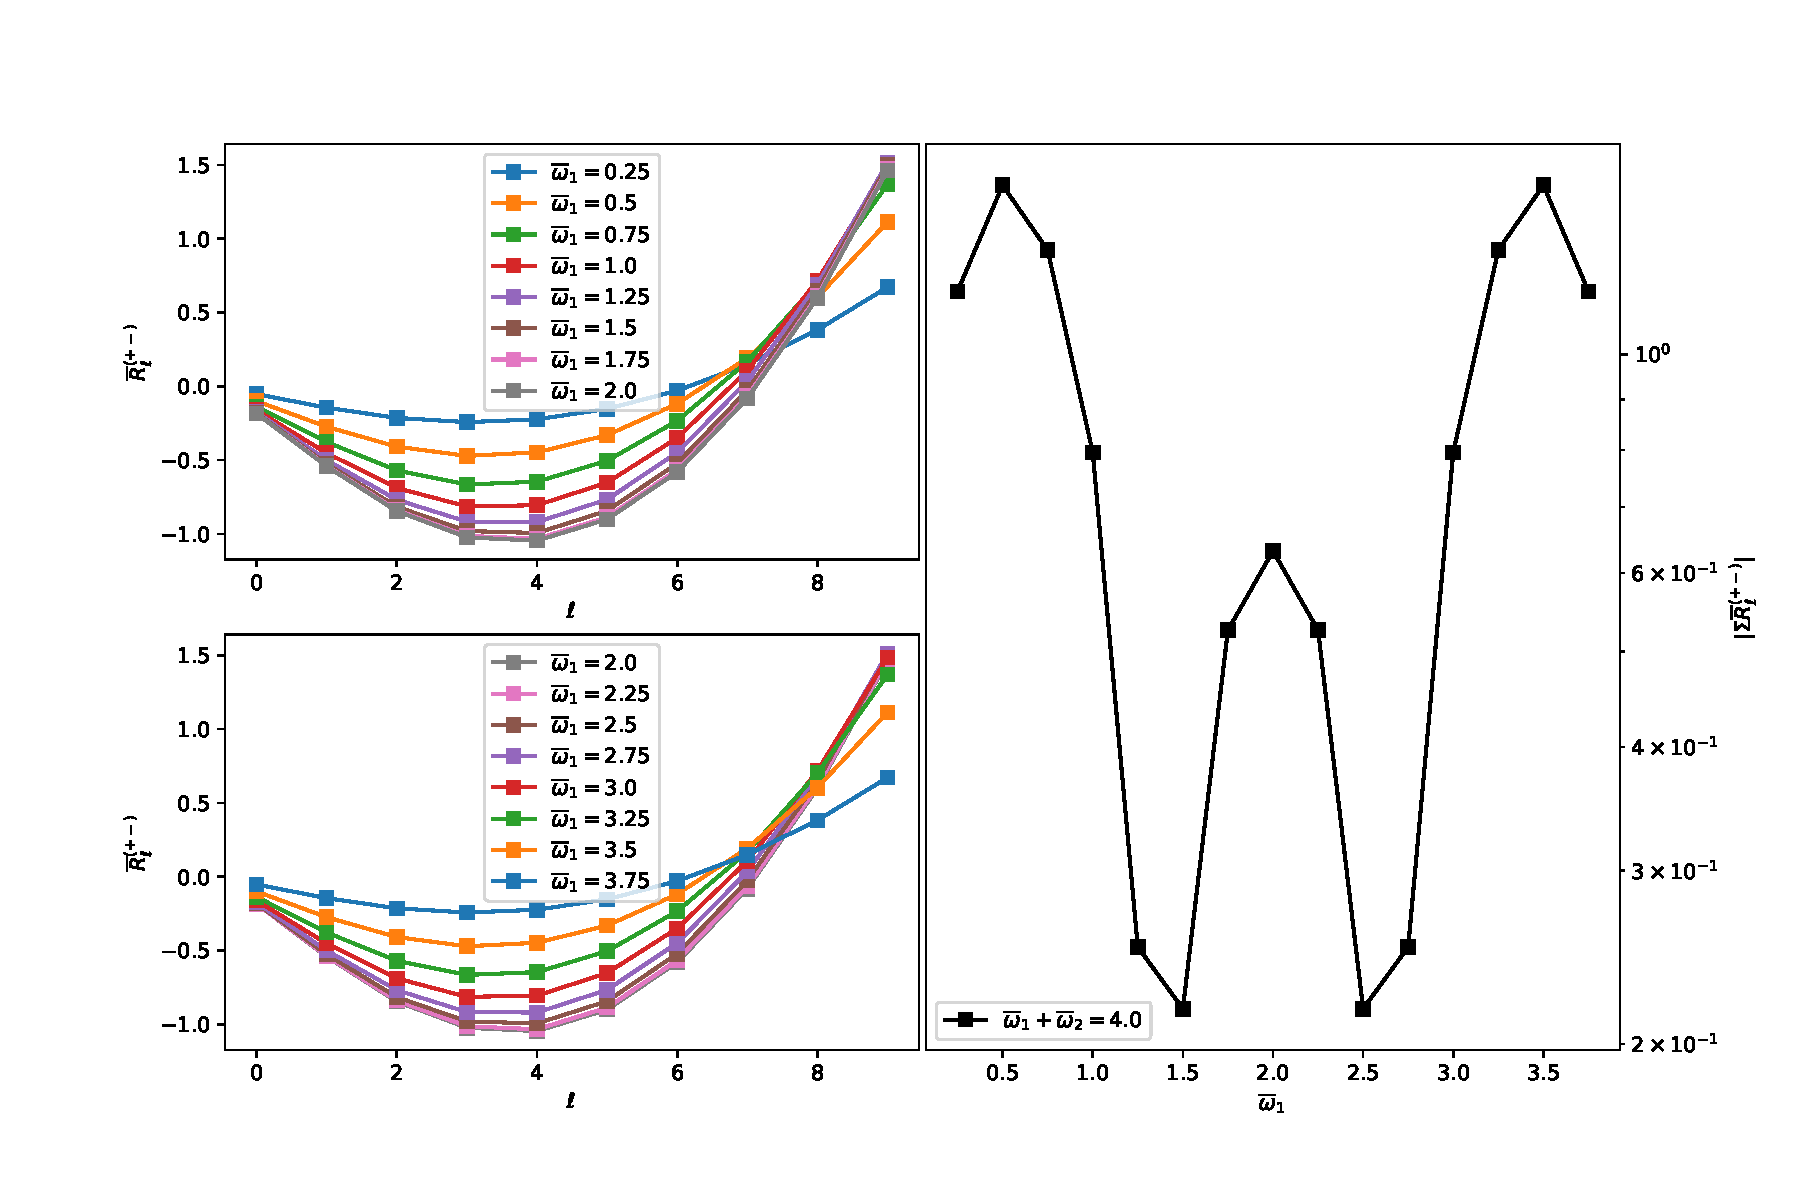
\includegraphics[width=\textwidth]{./figures/NN_equalfreq_pmchannel_n2_m0_0}
	\caption{$\overline{R}^{(+-)}_{(\ell - n)12\ell}$ for $m^2 = 0$.}
\end{figure}


\begin{figure}
\centering
	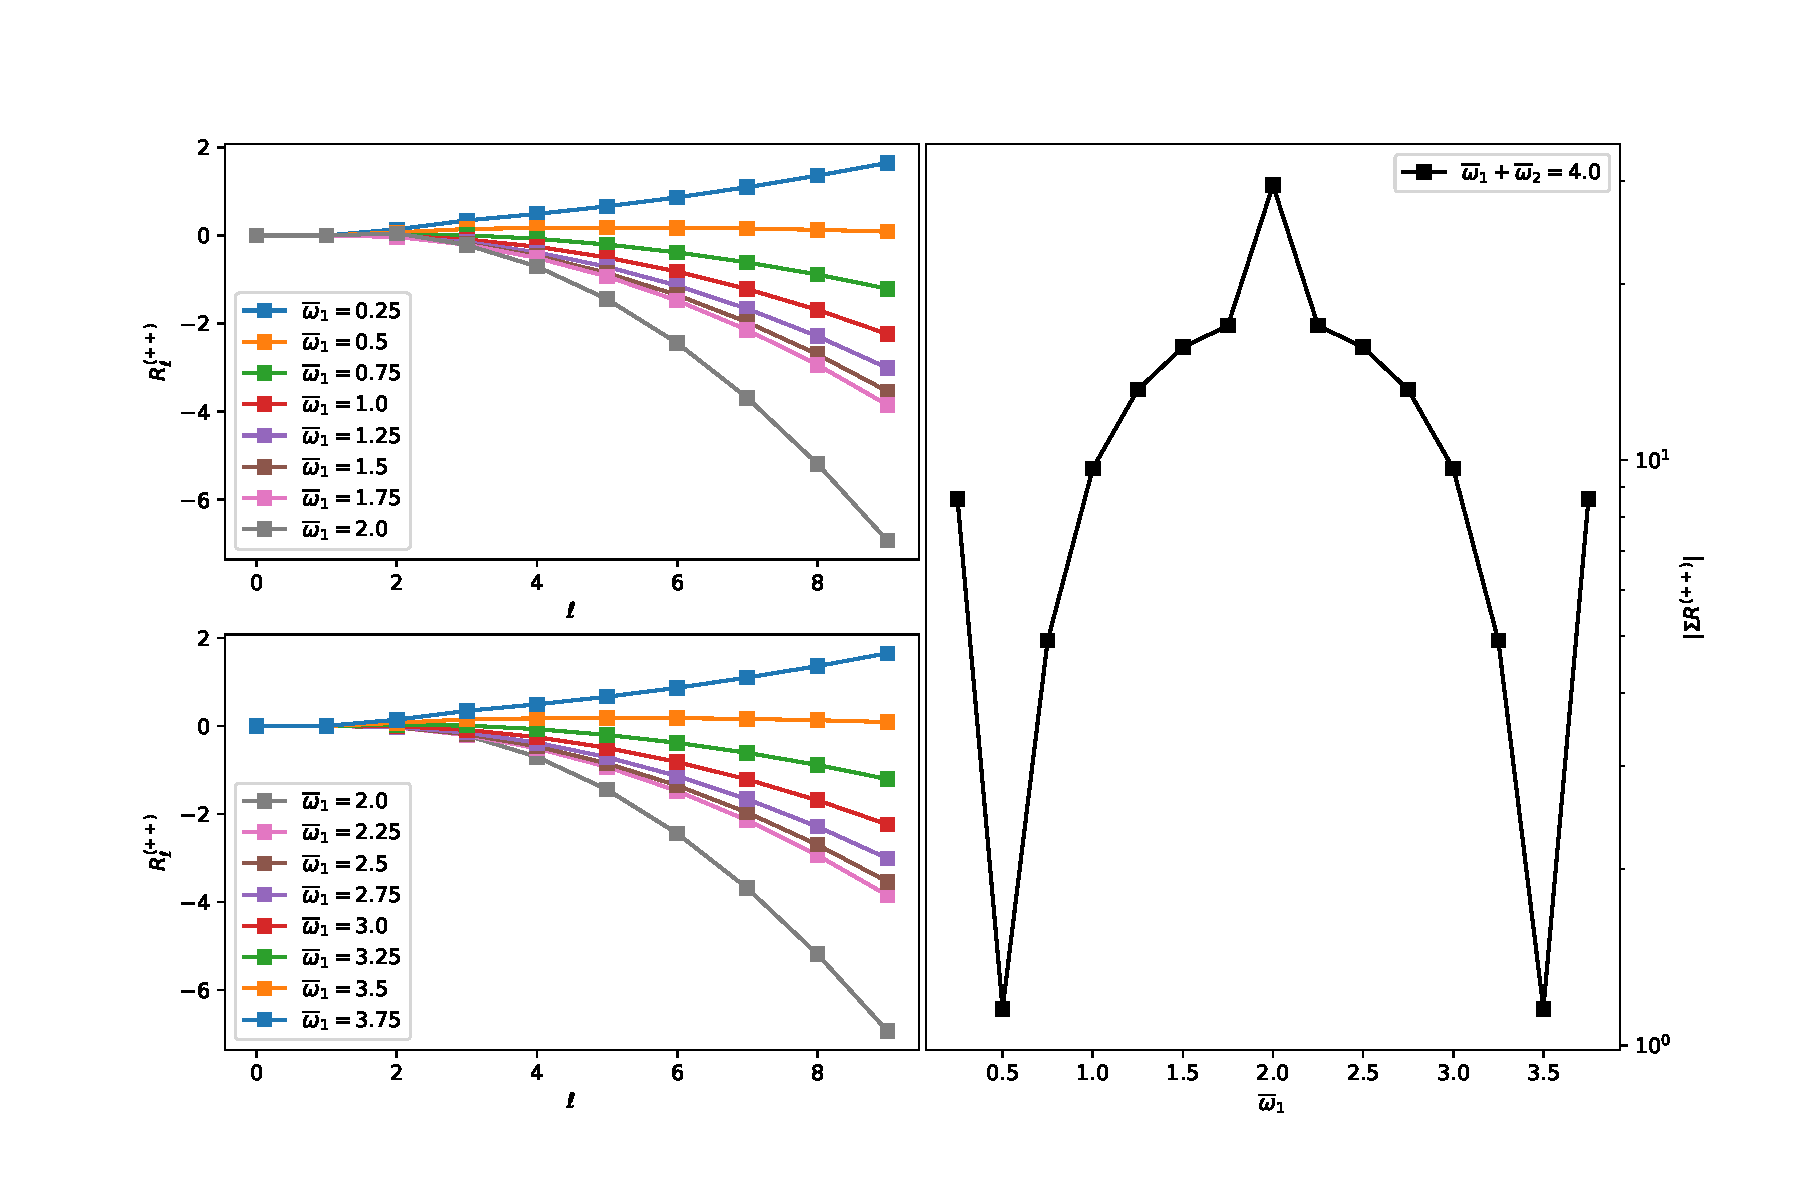
\includegraphics[width=\textwidth]{./figures/NN_equalfreq_ppchannel_n2_m-4_0}
	\caption{{\it Left, above}: Individual values of $\overline{R}^{(++)}_{(\ell - n)12\ell}$ for $m^2 = -4.0$ as a function of $\ell$ for $\oone + \otwo = 2n$ with $n = 4$ when $\oone \leq n$. {\it Left, below}: The same function, but for $\oone \geq n$; note the symmetry in values as $\oone \leftrightarrow \otwo$. {\it Right}: The absolute value of the sum of the $(++)$ source terms for choices of $\oone$.}
	\label{fig:atoi_pp_m-4_0}
\end{figure}

\begin{figure}
\centering
	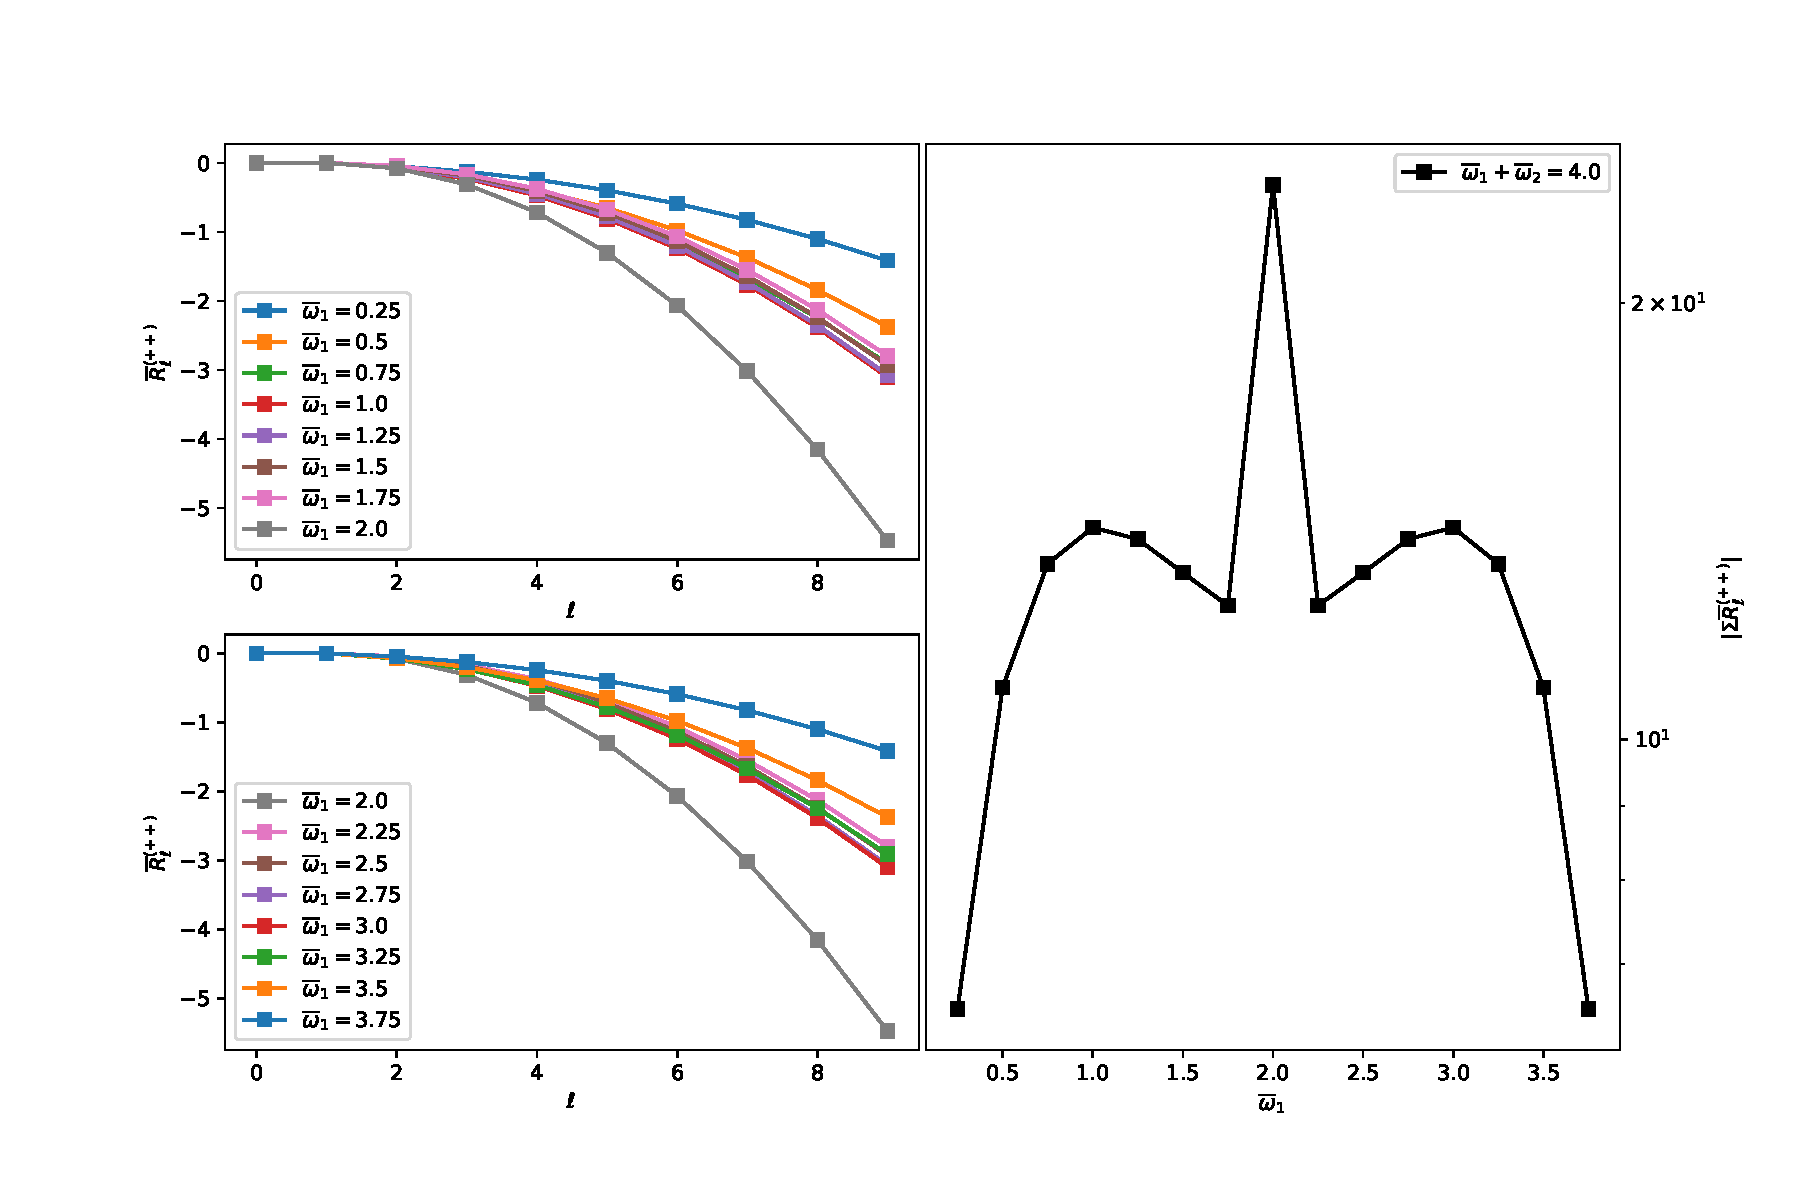
\includegraphics[width=\textwidth]{./figures/NN_equalfreq_ppchannel_n2_m0_0}
	\caption{$\overline{R}^{(++)}_{(\ell - n)12\ell}$ for $m^2 = 0$.}
\end{figure}


\subsubsection{$(++-)$}

This resonance channel\footnote{As is the case when all modes are normalizable, the results from this channel are equal to those from the $(+-+)$ channel under the exchange of $\ojb \leftrightarrow \okb$.} contributes secular terms to the $\mathcal{O}(\epsilon^3)$ source via:
\begin{align}
S_\ell &= \sum_{\jb, \kb}^{\jb \neq \kb} \overline{S}_{(\ell - \overline{j} + \overline{k}) \overline{j} \overline{k} \ell} \, \cos ( \theta_{(\ell - \overline{j} + \overline{k})} + \overline{\theta}_j - \overline{\theta}_k )  + \sum_{\jb}^{\jb \neq \ell} \overline{R}_{\overline{j} \ell} \, \cos \left( \theta_\ell + \overline{\theta}_j - \overline{\theta}_j \right) 
\end{align}
where
%\begin{align}
%\overline{T}_\ell &= \frac{1}{2} \ol^2 X_{\ell \ell \ell \ell} - \frac{3}{4} H_{\ell \ell \ell \ell} - \frac{9}{4} m^2 V_{\ell \ell \ell \ell} + 2 \ol^2 \widetilde{Z}^{+}_{\ell \ell \ell} - 2 \ol^4 P_{\ell \ell \ell} - \ol^2 M_{\ell \ell \ell} - m^2 \ol^2 Q_{\ell \ell \ell} \, ,
%\end{align}

\begin{align}
\overline{S}_{i \beta \gamma \ell} &= \frac{1}{4} \sum_{\gamma \neq \ell} \frac{\ogam}{\oi + \obet} Z^{-}_{i \beta \gamma \ell} + \frac{1}{4} \sum_{\beta \neq \ell} \frac{\obet}{\oi - \ogam} Z^+_{i \gamma \beta \ell} + \frac{1}{4} \sum_{i \neq \ell} \frac{\oi}{\obet - \ogam} Z^+_{\beta \gamma i \ell} \nonumber \\
%
& \quad + \frac{1}{4} \sum_{i \neq \gamma} \left[ \frac{\omega_\gamma}{\oi - \ogam} (H_{i \gamma \beta \ell} - 2\obet^2 X_{i \gamma \beta \ell}) - \frac{\oi}{\oi + \ogam} (H_{\gamma i \beta \ell} - 2\obet^2 X_{\gamma i \beta \ell} ) \right] \nonumber \\
%
& \quad + \frac{1}{4} \sum_{\beta \neq \gamma} \left[ \frac{\ogam}{\obet - \ogam} (H_{\beta \gamma i \ell} - 2 \oi^2 X_{\beta\gamma i \ell} ) - \frac{\obet}{\obet + \ogam} (H_{\gamma \beta i \ell} - 2\oi^2 X_{\gamma \beta i \ell} ) \right] \nonumber \\
%
& \quad -  \frac{1}{4} \sum_{i \neq \beta} \left[ \frac{\obet}{\oi + \obet} (H_{i \beta \gamma \ell} - 2\ogam^2 X_{i \beta \gamma \ell} ) + \frac{\oi}{\oi + \obet} (H_{\beta i \gamma \ell} - 2\ogam^2 X_{\beta i \gamma \ell}) \right] \nonumber \\
%
& \quad - \frac{1}{2} \sum \left( \obet \ogam X_{i \beta \gamma \ell} + \oi \ogam X_{\beta \gamma i \ell} - \oi \obet X_{\gamma i \beta \ell} \right) \, ,
\end{align}

\begin{align}
\overline{S}_{\alpha \beta k \ell} &= \frac{1}{4} \sum_{\alpha \neq \ell} \frac{\omega_\alpha}{\omega_\beta + \omega_k} Z^{-}_{\beta k \alpha \ell} + \frac{1}{4} \sum_{\beta \neq \ell} \frac{\omega_\beta}{\ok - \omega_{\alpha}} Z^{+}_{\alpha k \beta \ell} + \frac{1}{4} \sum_{k \neq \ell} \frac{\ok}{\obet - \omega_\alpha} Z^{+}_{\alpha \beta k \ell} \nonumber \\
%
& \quad + \frac{1}{4} \sum_{k \neq \alpha} \left[ \frac{\oal}{\ok - \oal} (H_{k \alpha \beta \ell} - 2 \obet^2 X_{k \alpha \beta \ell}) - \frac{\ok}{\ok + \oal} (H_{\alpha k \beta \ell} - 2\obet^2 X_{\alpha k \beta \ell}) \right] \nonumber \\
%
& \quad + \frac{1}{4} \sum_{\alpha \neq \beta} \left[ \frac{\oal}{\obet - \oal} (H_{\beta \alpha k \ell} - 2\ok^2 X_{\beta \alpha k \ell}) - \frac{\obet}{\oal + \obet}(H_{\alpha \beta k \ell} - 2 \ok^2 X_{\alpha \beta k \ell}) \right] \nonumber \\
%
& \quad - \frac{1}{4} \sum_{k \neq \beta} \left[ \frac{\obet}{\ok + \obet} (H_{k \beta \alpha \ell} - 2\oal^2 X_{k \beta \alpha \ell}) + \frac{\ok}{\ok + \obet}(H_{\beta k \alpha \ell} - 2\oal^2 X_{\beta k \alpha \ell}) \right] \nonumber \\
%
& \quad - \frac{1}{2} \sum \left( \oal \obet X_{k \alpha \beta \ell} + \oal \ok X_{\beta k \alpha \ell} - \obet \ok X_{\alpha \beta k \ell} \right) \, .
\end{align}

\begin{align}
\label{integer plus: ++- source}
\overline{S}_{i \jb \kb \ell} &= \frac{1}{2} Z^{+}_{\jb \kb i\ell} \left( \frac{\oi}{\ojb - \okb} \right) + \frac{1}{2} Z^{-}_{i \jb \kb \ell} \left( \frac{\okb}{\oi + \ojb} \right) + \frac{1}{2} Z^{+}_{i \kb \jb \ell} \left( \frac{\ojb}{\oi - \okb} \right) \nonumber \\
%
& \quad + \frac{1}{2} \ojb H_{i \jb \kb \ell} \left( \frac{1}{\oi - \ojb} - \frac{1}{\oi + \okb} \right) - \frac{1}{2} \oi H_{\jb i \kb \ell} \left( \frac{1}{\oi - \ojb} + \frac{1}{\oi + \okb} \right) \nonumber \\
%
& \quad - \frac{1}{2} \okb H_{\jb \kb i \ell} \left( \frac{1}{\ojb + \okb} - \frac{1}{\oi + \okb} \right) - \ojb \okb X_{i \jb \kb \ell} \left( \frac{\okb}{\oi - \ojb} - \frac{\ojb}{\oi + \okb} + 1 \right) \nonumber \\
%
& \quad + \oi \okb X_{\jb \kb i \ell} \left( \frac{\okb}{\oi - \ojb} + \frac{\oi}{\ojb + \okb} - 1 \right) + \oi \ojb X_{\kb i \jb \ell} \left( \frac{\ojb}{\oi + \okb} + \frac{\oi}{\ojb + \okb} + 1 \right) \nonumber \\
%
& \quad - m^2 V_{\kb i \jb \ell} \left( \frac{\oi}{\oi - \ojb} + \frac{\okb}{\ojb + \okb} + 1 \right) - m^2 V_{i \jb \kb \ell} \left( \frac{\oi}{\oi + \okb} + \frac{\ojb}{\ojb + \okb} + 1 \right) \nonumber \\
%
& \quad + m^2 V_{\jb \kb i \ell} \left( \frac{\ojb}{\oi - \ojb} - \frac{\okb}{\oi + \okb} - 1 \right) \, ,
\end{align}
\begin{align}
\overline{R}_{\jb i} &= \frac{1}{2} Z^{-}_{i \jb \jb \ell} \left( \frac{\ojb}{\oi + \ojb} \right) + \frac{1}{2} Z^{+}_{i \jb \jb \ell} \left( \frac{\ojb}{\oi - \ojb} \right) + \frac{1}{2} \left( \frac{\ojb}{\oi - \ojb} \right) H_{\jb \jb i \ell} - H_{\jb i \jb \ell} \left( \frac{\oi^2}{\oi^2 - \ojb^2} \right) \nonumber \\
%
& \quad - \frac{5}{4} H_{\jb \jb i \ell}  - \ojb^2 X_{i \jb \jb \ell} \left( \frac{\oi^2 + \ojb^2}{\oi^2 - \ojb^2} \right) + 3 \oi^2 X_{\jb \jb i \ell} + \oi \ojb X_{\jb \jb i \ell} \left( \frac{\ojb}{\oi^2 - \ojb^2} + \frac{\ojb}{\oi + \ojb} \right) \nonumber \\
%
& \quad -4m^2 V_{i \jb \jb \ell} - 2m^2 V_{i \jb \jb \ell} \left( \frac{\oi^2}{\oi^2 - \oj^2} \right) + 2m^2 V_{\jb \jb i \ell} \left( \frac{\ojb^2}{\oi^2 - \ojb^2} \right) - m^2 V_{\jb \jb i \ell} \nonumber \\
%
& \quad + 2\ojb^2 (\ol^2 P_{\jb \jb \ell} - 3 \oi^2 P_{i \ell \jb} ) + 2\ol^2 B_{\jb \jb \ell} + 2 \ojb^2 B_{i \ell \jb} \, .
\end{align}


%%%%%%%%%%%%%%%%%%%%%%%%
Sum of two NN frequencies is an integer:
\begin{align}
\overline{R}^{(1)}_{i \ell} &= \frac{1}{4} Z^{-}_{12i\ell} \left( \frac{2n - \ol}{2n} \right) - \frac{1}{4} Z^{-}_{i21\ell} \frac{\oone(\ol + \oone)}{\ol^2 - \oone^2} - \frac{1}{4} Z^{-}_{i12\ell} \frac{\otwo (\ol + \otwo)}{\ol^2 - \otwo^2} - \frac{1}{4}  \oone H_{i12\ell} \left( \frac{1}{\ol - \otwo} + \frac{1}{2n} \right) \nonumber \\
%
& \quad - \frac{1}{4} \otwo H_{i21\ell} \left( \frac{1}{\ol - \oone} + \frac{1}{2n} \right) - \frac{1}{4} (\ol - 2n) H_{1i2\ell} \left( \frac{1}{\ol - \oone} + \frac{1}{\ol - \otwo} \right) \nonumber \\
%
& \quad + \frac{1}{2} \oone \otwo X_{i12\ell} \left( \frac{\otwo}{\ol - \otwo} + \frac{\oone}{\ol - \oone} + 1 \right) + \frac{1}{2} (\ol - 2n) \otwo X_{12i\ell} \left( \frac{\otwo}{\ol - \otwo} + \frac{\ol}{2n} \right) \nonumber \\
%
& \quad + \frac{1}{2} (\ol - 2n) \oone X_{21i\ell} \left( \frac{\oone}{\ol - \oone} + \frac{\ol}{2n} \right) - \frac{m^2}{4} V_{12i\ell} \left( \frac{\oone}{\ol - \otwo} + \frac{\otwo}{\ol - \oone} + 1 \right) \nonumber \\
%
& \quad - \frac{m^2}{4} V_{i21\ell} \left( \frac{\ol - 2n}{\ol - \otwo} + \frac{\ol - 2n}{\ol - \oone} + 2 \right) - \frac{m^2}{4} V_{i12\ell} \, ,
\end{align}
\begin{align}
\overline{R}^{(2)}_{i \ell} &= \frac{1}{4} Z^{-}_{12i\ell} \left(\frac{\ol + 2n}{2n} \right) - \frac{1}{4} Z^{+}_{i 21\ell} \frac{\oone (\ol - \oone)}{\ol^2 - \oone^2} - \frac{1}{4} Z^{+}_{i12\ell} \frac{\otwo (\ol - \otwo)}{\ol^2 - \otwo^2} + \frac{1}{4} \oone H_{i12\ell} \left( \frac{1}{\ol + \otwo} - \frac{1}{2n} \right) \nonumber \\
%
& \quad + \frac{1}{4} \otwo H_{i21\ell} \left( \frac{1}{\ol + \oone} - \frac{1}{2n} \right) - \frac{1}{4} (\ol + 2n) H_{1i2\ell} \left( \frac{1}{\ol + \oone} + \frac{1}{\ol + \otwo} \right) \nonumber \\
%
& \quad - \frac{1}{2} \oone \otwo X_{i12\ell} \left( \frac{\otwo}{\ol + \otwo} + \frac{\oone}{\ol + \oone} - 1 \right) + \frac{1}{2} (\ol + 2n) \otwo X_{12i \ell} \left( \frac{\otwo}{\ol + \otwo} + \frac{\ol}{2n} \right) \nonumber \\
%
& \quad + \frac{1}{2} (\ol + 2n) \oone X_{21i\ell} \left( \frac{\oone}{\ol + \oone} + \frac{\ol}{2n} \right) + \frac{m^2}{4} V_{12i\ell} \left( \frac{\oone}{\ol + \otwo} + \frac{\otwo}{\ol + \oone} -1 \right) \nonumber \\
%
& \quad - \frac{m^2}{4} V_{i21\ell} \left( \frac{\ol + 2n}{\ol + \otwo} + \frac{\otwo}{2n} + 1\right) - \frac{m^2}{4} V_{i12\ell} \left( \frac{\ol + 2n}{\ol + \oone} + \frac{\oone}{2n} + 1 \right) \, .
\end{align}

